% body_diode_lauritzen_ma.tex
% The body diode of a power MOSFET as a Lauritzen-Ma diode: parameter extraction from the datasheet of the MOSFET
% pwr-control template (AAA_template_latex_settings); numbers and figures of the worked examples:
% body_diode_calc.py (with the module body_diode_lm.py, which imports lm_conversion.py of the note
% research/power_semiconductor_devices/diode/lauritzen_ma_datasheet_conversion), which writes body_diode_values.tex
% Compile: pdflatex body_diode_lauritzen_ma.tex  (twice, for references)
% Rev. 00 - November 2026 - first issue
\documentclass[10pt,a4paper]{scrartcl}
\input{../../../../AAA_template_latex_settings/settings}
% the document sits four levels below the repository root: logo path of settings.tex corrected here
\rhead{\includegraphics[height=0.75cm]{../../../../AAA_template_latex_settings/pwr-control_logo_doc.png}}
\rfoot{\small Rev.~00}
\geometry{left=2.0cm, right=2.0cm}
\usepackage[european resistors, american inductors]{circuitikz}
\usetikzlibrary{patterns, arrows.meta, positioning}

\sisetup{per-mode=symbol,range-phrase={\text{--}},range-units=single}
\setlist{nosep}
\setlength{\parindent}{0pt}
\setlength{\parskip}{3pt}
\allowdisplaybreaks
\captionsetup{font=small,labelfont=bf}
\renewcommand{\topfraction}{0.9}
\renewcommand{\bottomfraction}{0.9}
\renewcommand{\textfraction}{0.05}
\renewcommand{\floatpagefraction}{0.8}

% --- numbers of the worked examples (generated by body_diode_calc.py) ---
% generated by body_diode_calc.py: do not edit by hand
\newcommand{\bdIptCzero}{15.9}
\newcommand{\bdIptM}{0.91}
\newcommand{\bdIptVj}{5}
\newcommand{\bdIptQoss}{213}
\newcommand{\bdIptCapIrrm}{6.5}
\newcommand{\bdIptCapTrr}{65}
\newcommand{\bdIptVr}{50}
\newcommand{\bdIptIf}{100}
\newcommand{\bdIptSlope}{100}
\newcommand{\bdIptCoss}{1800}
\newcommand{\bdIptVds}{100}
\newcommand{\bdIptRdson}{1.5}
\newcommand{\bdIrfCzero}{3.0}
\newcommand{\bdIrfM}{0.63}
\newcommand{\bdIrfVj}{5}
\newcommand{\bdIrfQoss}{79}
\newcommand{\bdIrfCapIrrm}{4.0}
\newcommand{\bdIrfCapTrr}{40}
\newcommand{\bdIrfVr}{85}
\newcommand{\bdIrfIf}{75}
\newcommand{\bdIrfSlope}{100}
\newcommand{\bdIrfCoss}{670}
\newcommand{\bdIrfVds}{100}
\newcommand{\bdIrfRdson}{4.5}
\newcommand{\bdStpCzero}{2.1}
\newcommand{\bdStpM}{0.50}
\newcommand{\bdStpVj}{1}
\newcommand{\bdStpQoss}{33}
\newcommand{\bdStpCapIrrm}{2.6}
\newcommand{\bdStpCapTrr}{26}
\newcommand{\bdStpVr}{80}
\newcommand{\bdStpIf}{32}
\newcommand{\bdStpSlope}{100}
\newcommand{\bdStpCoss}{290}
\newcommand{\bdStpVds}{100}
\newcommand{\bdStpRdson}{24.0}
\newcommand{\bdIptQrr}{316}
\newcommand{\bdIptQrrMax}{632}
\newcommand{\bdIptTrr}{103}
\newcommand{\bdIptTrrMax}{206}
\newcommand{\bdIptQossMax}{284}
\newcommand{\bdIptQossPct}{67}
\newcommand{\bdIptQossMaxPct}{45}
\newcommand{\bdIptQdif}{103}
\newcommand{\bdIptQdifMax}{348}
\newcommand{\bdIptQdifPct}{33}
\newcommand{\bdIrfLoT}{25}
\newcommand{\bdIrfLoQrr}{94}
\newcommand{\bdIrfLoTrr}{50}
\newcommand{\bdIrfLoQdif}{15}
\newcommand{\bdIrfLoQossPct}{84}
\newcommand{\bdIrfLoQrrMax}{140}
\newcommand{\bdIrfLoTrrMax}{75}
\newcommand{\bdIrfHiT}{125}
\newcommand{\bdIrfHiQrr}{140}
\newcommand{\bdIrfHiTrr}{60}
\newcommand{\bdIrfHiQdif}{61}
\newcommand{\bdIrfHiQossPct}{56}
\newcommand{\bdIrfHiQrrMax}{210}
\newcommand{\bdIrfHiTrrMax}{90}
\newcommand{\bdIrfIrrm}{3.5}
\newcommand{\bdIrfTri}{61}
\newcommand{\bdIrfQdifRatio}{4.0}
\newcommand{\bdIrfTauRatio}{2.0}
\newcommand{\bdStpQrr}{47}
\newcommand{\bdStpTrr}{41}
\newcommand{\bdStpIrrm}{2.3}
\newcommand{\bdStpT}{150}
\newcommand{\bdStpQdif}{14}
\newcommand{\bdStpQossPct}{71}
\newcommand{\bdStpTri}{26}
\newcommand{\bdStpMassumed}{0.5}
\newcommand{\bdIptIrr}{3.75}
\newcommand{\bdIptTa}{37.5}
\newcommand{\bdIptTaurr}{8.7}
\newcommand{\bdIptTc}{65}
\newcommand{\bdIptTau}{46}
\newcommand{\bdIptTauOne}{46.2}
\newcommand{\bdIptTm}{11}
\newcommand{\bdIptTmOne}{10.7}
\newcommand{\bdIptTauL}{46.2}
\newcommand{\bdIptTmL}{10.7}
\newcommand{\bdIptIter}{2}
\newcommand{\bdIptX}{22}
\newcommand{\bdIptLam}{22}
\newcommand{\bdIptS}{0.46}
\newcommand{\bdIptRho}{0.19}
\newcommand{\bdIptQtri}{70}
\newcommand{\bdIptQtail}{33}
\newcommand{\bdIptConvSpread}{0.00}
\newcommand{\bdIptIres}{2.0}
\newcommand{\bdIptTzero}{1}
\newcommand{\bdIptRampIrrm}{10.3}
\newcommand{\bdIptRampTri}{530}
\newcommand{\bdIptSQuarterIrr}{4.06}
\newcommand{\bdIptSQuarterTau}{46}
\newcommand{\bdIptSQuarterTm}{6}
\newcommand{\bdIptSQuarterTrrP}{98}
\newcommand{\bdIptSQuarterTrrR}{79}
\newcommand{\bdIptSQuarterIrrmR}{7.9}
\newcommand{\bdIptSHalfIrr}{3.71}
\newcommand{\bdIptSHalfTau}{46}
\newcommand{\bdIptSHalfTm}{12}
\newcommand{\bdIptSHalfTrrP}{104}
\newcommand{\bdIptSHalfTrrR}{79}
\newcommand{\bdIptSHalfIrrmR}{7.9}
\newcommand{\bdIptSOneIrr}{3.21}
\newcommand{\bdIptSOneTau}{48}
\newcommand{\bdIptSOneTm}{24}
\newcommand{\bdIptSOneTrrP}{114}
\newcommand{\bdIptSOneTrrR}{79}
\newcommand{\bdIptSOneIrrmR}{7.9}
\newcommand{\bdIptSTwoIrr}{2.62}
\newcommand{\bdIptSTwoTau}{52}
\newcommand{\bdIptSTwoTm}{52}
\newcommand{\bdIptSTwoTrrP}{133}
\newcommand{\bdIptSTwoTrrR}{78}
\newcommand{\bdIptSTwoIrrmR}{7.8}
\newcommand{\bdIptNIrr}{5.0}
\newcommand{\bdIptNTau}{88}
\newcommand{\bdIptNTm}{68}
\newcommand{\bdIptNTaurr}{38}
\newcommand{\bdIptNTriIrr}{6.1}
\newcommand{\bdIptNTriTau}{82}
\newcommand{\bdIptNTriTm}{28}
\newcommand{\bdIptNTriTaurr}{21}
\newcommand{\bdIptNTenIrr}{6.5}
\newcommand{\bdIptNTenTau}{81}
\newcommand{\bdIptNTenTm}{21}
\newcommand{\bdIptNTenTaurr}{17}
\newcommand{\bdIptKtwentyfive}{1.39}
\newcommand{\bdIptNTauRatio}{1.9}
\newcommand{\bdIptNTmRatio}{6.3}
\newcommand{\bdIptNQrrDouble}{529}
\newcommand{\bdIptNQrrDoublePct}{67}
\newcommand{\bdIptXIrr}{3.0}
\newcommand{\bdIptXTaurr}{99}
\newcommand{\bdIptXTau}{130}
\newcommand{\bdIptXTm}{422}
\newcommand{\bdIptXS}{6.51}
\newcommand{\bdIptXTauRatio}{2.8}
\newcommand{\bdIptDcm}{18}
\newcommand{\bdIptLdiff}{9}
\newcommand{\bdIptWpar}{15}
\newcommand{\bdIptWstore}{13}
\newcommand{\bdIptWlo}{6}
\newcommand{\bdIptWhi}{10}
\newcommand{\bdIptTlo}{10}
\newcommand{\bdIptThi}{28}
\newcommand{\bdIptTmGeom}{3.0}
\newcommand{\bdIptIsTwo}{1.4\times10^{-5}}
\newcommand{\bdIptIsStarTwo}{1.8\times10^{-5}}
\newcommand{\bdIptVtenTwo}{0.70}
\newcommand{\bdIptVthreeTwo}{0.99}
\newcommand{\bdIptIsOne}{2.0\times10^{-12}}
\newcommand{\bdIptIsStarOne}{2.5\times10^{-12}}
\newcommand{\bdIptVtenOne}{0.75}
\newcommand{\bdIptVthreeOne}{0.96}
\newcommand{\bdIptVt}{25.7}
\newcommand{\bdIptRs}{0.4}
\newcommand{\bdIptVsd}{0.85}
\newcommand{\bdIptVsdMax}{1.2}
\newcommand{\bdIptIvsd}{100}
\newcommand{\bdIptN}{2}
\newcommand{\bdIptIsFactor}{1.23}
\newcommand{\bdIptRr}{100}
\newcommand{\bdIptRrHot}{1}
\newcommand{\bdIptChVHundred}{150}
\newcommand{\bdIptChIHundred}{2.5\times10^{-4}}
\newcommand{\bdIptChQHundred}{1.2\times10^{-11}}
\newcommand{\bdIptChVThree}{450}
\newcommand{\bdIptChIThree}{9.0\times10^{-2}}
\newcommand{\bdIptChQThree}{4.2\times10^{-9}}
\newcommand{\bdIptExpIa}{1.00}
\newcommand{\bdIptExpQa}{1.00}
\newcommand{\bdIptSimPTone}{43}
\newcommand{\bdIptSimPTtwo}{97}
\newcommand{\bdIptSimPIrrm}{4.3}
\newcommand{\bdIptSimPQrr}{339}
\newcommand{\bdIptSimPTrr}{101}
\newcommand{\bdIptSimPTrrLine}{102}
\newcommand{\bdIptSimPVpk}{58}
\newcommand{\bdIptSimPQrrErr}{+7}
\newcommand{\bdIptSimPTrrErr}{-2}
\newcommand{\bdIptSimRTone}{43}
\newcommand{\bdIptSimRTtwo}{81}
\newcommand{\bdIptSimRIrrm}{8.1}
\newcommand{\bdIptSimRQrr}{350}
\newcommand{\bdIptSimRTrr}{85}
\newcommand{\bdIptSimRTrrLine}{86}
\newcommand{\bdIptSimRVpk}{65}
\newcommand{\bdIptSimRQrrErr}{+11}
\newcommand{\bdIptSimRTrrErr}{-17}
\newcommand{\bdIptSimQfwd}{13}
\newcommand{\bdIptSimQover}{13}
\newcommand{\bdIptVjzero}{0.81}
\newcommand{\bdIptRefTau}{42}
\newcommand{\bdIptRefTm}{13}
\newcommand{\bdIptRefTauErr}{-10}
\newcommand{\bdIptRefTmErr}{+23}
\newcommand{\bdIptRefQrr}{316}
\newcommand{\bdIptRefTrr}{103}
\newcommand{\bdIptRefIrrm}{3.8}
\newcommand{\bdIptRefTaurr}{10.0}
\newcommand{\bdIptRefNsim}{6}
\newcommand{\bdIptRefS}{0.52}
\newcommand{\bdIptXScale}{1.8}
\newcommand{\bdIptAltCzero}{29}
\newcommand{\bdIptAltM}{0.70}
\newcommand{\bdIptAltTau}{41}
\newcommand{\bdIptAltTm}{19}
\newcommand{\bdIptAltTauErr}{-2}
\newcommand{\bdIptAltTmErr}{+44}
\newcommand{\bdIptRefRIrrm}{7.8}
\newcommand{\bdIptRefRQrr}{328}
\newcommand{\bdIptRefRTrr}{82}
\newcommand{\bdIptNSimQrr}{523}
\newcommand{\bdIptNSimQrrErr}{+65}
\newcommand{\bdIptNSimTrr}{121}
\newcommand{\bdIptNSimIrrm}{5.8}
\newcommand{\bdIptCapSimIrrm}{6.6}
\newcommand{\bdIptCapSimQrr}{241}
\newcommand{\bdIptCapSimTrr}{71}
\newcommand{\bdIptLs}{10}
\newcommand{\bdIptRser}{1.0}
\newcommand{\bdAppTau}{42}
\newcommand{\bdAppTm}{13}
\newcommand{\bdAppRho}{0.24}
\newcommand{\bdAppLamDs}{24}
\newcommand{\bdAppQdsTdTwenty}{82.0}
\newcommand{\bdAppVbus}{48}
\newcommand{\bdAppQoss}{209}
\newcommand{\bdAppDsIrr}{3.2}
\newcommand{\bdAppDsQ}{82}
\newcommand{\bdAppDsQoverQoss}{0.4}
\newcommand{\bdAppDsSlope}{0.1}
\newcommand{\bdAppHalfTwentyIrr}{15.6}
\newcommand{\bdAppHalfTwentyQ}{400}
\newcommand{\bdAppHalfTwentyQPct}{98}
\newcommand{\bdAppHalfFiftyIrr}{15.7}
\newcommand{\bdAppHalfFiftyQ}{404}
\newcommand{\bdAppHalfFiftyQPct}{99}
\newcommand{\bdAppHalfHundredIrr}{15.8}
\newcommand{\bdAppHalfHundredQ}{406}
\newcommand{\bdAppHalfHundredQPct}{100}
\newcommand{\bdAppHalfLam}{4.79}
\newcommand{\bdAppHalfIrr}{15.8}
\newcommand{\bdAppHalfQ}{407}
\newcommand{\bdAppHalfQRatio}{5.0}
\newcommand{\bdAppHalfQoverQoss}{1.9}
\newcommand{\bdAppHalfSlope}{0.5}
\newcommand{\bdAppHalfX}{5.55}
\newcommand{\bdAppOneTwentyIrr}{28.0}
\newcommand{\bdAppOneTwentyQ}{674}
\newcommand{\bdAppOneTwentyQPct}{88}
\newcommand{\bdAppOneFiftyIrr}{29.2}
\newcommand{\bdAppOneFiftyQ}{720}
\newcommand{\bdAppOneFiftyQPct}{94}
\newcommand{\bdAppOneHundredIrr}{30.0}
\newcommand{\bdAppOneHundredQ}{750}
\newcommand{\bdAppOneHundredQPct}{98}
\newcommand{\bdAppOneLam}{2.40}
\newcommand{\bdAppOneIrr}{30.3}
\newcommand{\bdAppOneQ}{763}
\newcommand{\bdAppOneQRatio}{9.3}
\newcommand{\bdAppOneQoverQoss}{3.6}
\newcommand{\bdAppOneSlope}{1.0}
\newcommand{\bdAppOneX}{3.12}
\newcommand{\bdAppTwoTwentyIrr}{43.6}
\newcommand{\bdAppTwoTwentyQ}{914}
\newcommand{\bdAppTwoTwentyQPct}{73}
\newcommand{\bdAppTwoFiftyIrr}{48.9}
\newcommand{\bdAppTwoFiftyQ}{1088}
\newcommand{\bdAppTwoFiftyQPct}{87}
\newcommand{\bdAppTwoHundredIrr}{52.0}
\newcommand{\bdAppTwoHundredQ}{1198}
\newcommand{\bdAppTwoHundredQPct}{96}
\newcommand{\bdAppTwoLam}{1.20}
\newcommand{\bdAppTwoIrr}{53.3}
\newcommand{\bdAppTwoQ}{1244}
\newcommand{\bdAppTwoQRatio}{15.2}
\newcommand{\bdAppTwoQoverQoss}{5.9}
\newcommand{\bdAppTwoSlope}{2.0}
\newcommand{\bdAppTwoX}{1.84}
\newcommand{\bdAppIrrAbrupt}{316}
\newcommand{\bdAppQAbrupt}{3169}
\newcommand{\bdAppTdTwenty}{20}
\newcommand{\bdAppTdFifty}{50}
\newcommand{\bdAppTdHundred}{100}
\newcommand{\bdAppFillTwenty}{38}
\newcommand{\bdAppFillFifty}{70}
\newcommand{\bdAppFillHundred}{91}
\newcommand{\bdIrfHiIrr}{3.2}
\newcommand{\bdIrfHiTaurr}{3.5}
\newcommand{\bdIrfHiTau}{35}
\newcommand{\bdIrfHiTm}{3.9}
\newcommand{\bdIrfHiS}{0.22}
\newcommand{\bdIrfLoTau}{18}
\newcommand{\bdIrfLoIrr}{1.6}
\newcommand{\bdIrfCossTr}{950}
\newcommand{\bdIrfCossEr}{820}
\newcommand{\bdIrfCossTrV}{80}
\newcommand{\bdIrfQossEighty}{76}
\newcommand{\bdStpIrr}{1.4}
\newcommand{\bdStpTaurr}{3.2}
\newcommand{\bdStpTau}{17}
\newcommand{\bdStpTm}{3.9}
\newcommand{\bdStpS}{0.46}
\newcommand{\bdIptQrrR}{474.00}
\newcommand{\bdIptQossR}{319.50}
\newcommand{\bdIrfQrrR}{423.00}
\newcommand{\bdIrfQossR}{353.25}
\newcommand{\bdStpQrrR}{1128.00}
\newcommand{\bdStpQossR}{795.27}
\newcommand{\bdPEndPct}{2}


% --- shorthand (the notation of the note lauritzen_ma_datasheet_conversion) ---
\newcommand{\IF}{I_\mathrm{F}}
\newcommand{\VR}{V_\mathrm{R}}
\newcommand{\Irr}{I_\mathrm{rr}}
\newcommand{\Irrm}{I_\mathrm{rrm}}
\newcommand{\Qrr}{Q_\mathrm{rr}}
\newcommand{\Qdif}{Q_\mathrm{dif}}
\newcommand{\Qoss}{Q_\mathrm{oss}}
\newcommand{\Coss}{C_\mathrm{oss}}
\newcommand{\Crss}{C_\mathrm{rss}}
\newcommand{\Cds}{C_\mathrm{ds}}
\newcommand{\Cgd}{C_\mathrm{gd}}
\newcommand{\trr}{t_\mathrm{rr}}
\newcommand{\ta}{t_\mathrm{a}}
\newcommand{\tb}{t_\mathrm{b}}
\newcommand{\td}{t_\mathrm{d}}
\newcommand{\Tc}{T_\mathrm{c}}
\newcommand{\taurr}{\tau_\mathrm{rr}}
\newcommand{\TM}{T_\mathrm{M}}
\newcommand{\Tone}{T_1}
\newcommand{\Ttwo}{T_2}
\newcommand{\qE}{q_\mathrm{E}}
\newcommand{\qM}{q_\mathrm{M}}
\newcommand{\idif}{i_\mathrm{dif}}
\newcommand{\ic}{i_\mathrm{c}}
\newcommand{\ich}{i_\mathrm{ch}}
\newcommand{\vj}{v_\mathrm{j}}
\newcommand{\IS}{I_\mathrm{S}}
\newcommand{\RS}{R_\mathrm{S}}
\newcommand{\Rr}{R_\mathrm{r}}
\newcommand{\Rds}{R_\mathrm{DS(on)}}
\newcommand{\VT}{V_\mathrm{T}}
\newcommand{\VSD}{V_\mathrm{SD}}
\newcommand{\VDS}{V_\mathrm{DS}}
\newcommand{\Vj}{V_\mathrm{j}}
\newcommand{\Czero}{C_0}
\newcommand{\Ls}{L_\mathrm{s}}
\newcommand{\Rser}{R_\mathrm{s}}
\newcommand{\Tj}{T_\mathrm{j}}
\newcommand{\diff}{\mathrm{d}}
\newcommand{\ns}{\si{\nano\second}}
\newcommand{\nC}{\si{\nano\coulomb}}
\newcommand{\Aus}{\si{\ampere\per\micro\second}}
\newcommand{\Ans}{\si{\ampere\per\nano\second}}
\newcommand{\IPT}{IPT015N10N5}
\newcommand{\IRF}{IRFB4110}
\newcommand{\STP}{STP30N10F7}
\newcommand{\lmnote}{\texttt{lauritzen\_ma\_datasheet\_conversion}}

% =============================================================
%  DOCUMENT DATA (title page: AAA_template_latex_settings/titlepage.tex)
% =============================================================
\newcommand{\DocCategory}{Technical Note}
\newcommand{\DocField}{Power Electronics and Control Systems}
\newcommand{\DocTitle}{%
	{\fontsize{20}{24}\selectfont\bfseries The Body Diode of a Power MOSFET} \\[16pt]
	{\fontsize{16}{20}\selectfont\bfseries as a Lauritzen--Ma Diode}
}
\newcommand{\DocSubtitle}{Parameter extraction from the datasheet of a low-voltage MOSFET: the output charge taken apart from the stored charge, the recovery test seen at the terminals, the channel in parallel}
\newcommand{\DocAuthor}{Davide Bagnara}
\newcommand{\DocRevision}{00}
\newcommand{\DocDate}{November 2026}
\newcommand{\DocAbstract}{%
The body diode of a power MOSFET is a PIN diode: the p-body, the drift region and the substrate. In a converter it conducts during the dead time and recovers when the opposite switch turns on, and a circuit simulation needs a diode model that stores charge. The Lauritzen--Ma model does it with two parameters, the lifetime $\tau$ and the transit time $\TM$; the datasheet of a MOSFET gives a recovery time and a recovered charge at one test condition, sometimes a peak current, and nothing else. This note shows how to get from one to the other. The difference from a discrete diode is the output capacitance: for a low-voltage MOSFET the charge $\Qoss(\VR)$ that it takes during the test is one half to five sixths of the datasheet $\Qrr$, and the capacitance alone produces a recovery-like waveform with a peak of a few amperes. Only the difference $\Qrr - \Qoss(\VR)$ is stored charge, and what the peak current and the recovery time contain depends on the driver of the test, which the datasheet does not describe. The note derives the recovery test at the terminals for two driver models, gives the conversion from the stored charge and the recovery time, brackets the result when only the charge is known, and checks it in a simulated test with the complete device. Three real datasheets are worked through: a 100~V trench MOSFET in full, a planar one at two temperatures and a small trench one at \SI{150}{\celsius}. For the trench MOSFET the lifetime is about \SI{\bdIptRefTau}{\nano\second} and the transit time about \SI{\bdIptRefTm}{\nano\second}; the set obtained without subtracting the output charge counts it twice and returns a charge \SI{\bdIptNSimQrrErr}{\percent} too high. The note closes with the channel in parallel (no charge is stored while it conducts; a dead time shorter than the lifetime matters only on fast ramps), the temperature, the slope of the application, and the devices for which the model is not the right tool. The companion Python scripts reproduce every number and figure.
}
\newcommand{\RevisionHistory}{%
	00 & November 2026 & First issue. & \DocAuthor \\
}
\newcommand{\MetaLabelA}{Project Repository}
\newcommand{\MetaValueAUrl}{https://github.com/pwr-control/repositories-documentation.git}
\newcommand{\MetaValueALabel}{repositories-documentation.git}
\newcommand{\MetaLabelB}{Calculation}
\newcommand{\MetaValueB}{Python 3 / NumPy, SciPy (\texttt{body\_diode\_calc.py})}

\begin{document}
\input{../../../../AAA_template_latex_settings/titlepage}
\tableofcontents
\newpage

%=====================================================================
\section{Scope and results}
\label{sec:scope}
A power MOSFET conducts in the third quadrant through two paths: the channel, when the gate is on, and the body diode, the p-n junction between the p-body and the n-type drift region. In a half-bridge the body diode carries the load current during the dead time, and when the opposite switch turns on it recovers like any PIN diode: a reverse current flows until the stored charge is gone. The recovery adds to the turn-on loss of the opposite switch, rings with the stray inductance and, in some devices, is the dominant loss of synchronous rectification. A circuit simulation of the leg needs a body-diode model that stores charge.

The model of Lauritzen and Ma \cite{lauritzen1991} is the simplest one that does it with a soft tail. It has two recovery parameters, the lifetime $\tau$ and the transit time $\TM$, and the note \lmnote{} of this repository \cite{lmnote} derives how they relate to the data of a diode datasheet: the peak reverse recovery current $\Irr$, the recovered charge $\Qrr$ and the recovery time $\trr$ at a test condition. This note applies that conversion to the body diode of a MOSFET, where three things are different:
\begin{itemize}
\item the diode sits in parallel with the output capacitance $\Coss$ of the MOSFET, which is large, and the reverse recovery test charges it: the datasheet $\Qrr$ contains the output charge $\Qoss(\VR)$, and for a low-voltage device this is most of it;
\item the diode sits in parallel with the channel, which decides how much charge is stored before a commutation;
\item the datasheet gives less: often no peak current, no definition of the recovery time, no second temperature, and the values are typical ones ``defined by design''.
\end{itemize}
The note is written to stand alone: Sec.~\ref{sec:model} recalls the model and the conversion of \cite{lmnote} in the form needed here, and the proofs are in that note. Section~\ref{sec:body} describes the body diode, Sec.~\ref{sec:datasheet} what the datasheet gives, Sec.~\ref{sec:coss} the output capacitance in the recovery test, Sec.~\ref{sec:extraction} the extraction, Sec.~\ref{sec:example} the worked example and its check in a simulated test, Secs.~\ref{sec:channel} to~\ref{sec:limits} the channel, the temperature, the slope of the application and the limits, and Sec.~\ref{sec:procedure} the procedure. Three datasheets are used (Table~\ref{tab:data}): \IPT{} (Infineon OptiMOS~5, \SI{100}{\volt}, trench) \cite{ipt}, worked in full; \IRF{} (planar HEXFET, \SI{100}{\volt}, two temperatures and a peak current given) \cite{irf}; \STP{} (ST STripFET~F7, \SI{100}{\volt}, data at \SI{150}{\celsius}) \cite{stp}. They were chosen for what their datasheets print, not as a recommendation; to convert another device, the data at the top of \texttt{body\_diode\_calc.py} are replaced.

\subsection*{The results in short}
\begin{enumerate}
\item The reverse recovery test of a MOSFET charges $\Coss$ to $\VR$ while the current is reversed, so the datasheet charge is the stored charge plus the output charge: $\Qrr = \Qdif + \Qoss(\VR)$, \eqref{eq:balance}. For the three devices $\Qoss(\VR)$ is \SI{\bdIptQossPct}{\percent}, \SI{\bdIrfLoQossPct}{\percent} and \SI{\bdStpQossPct}{\percent} of the typical $\Qrr$ (Fig.~\ref{fig:floor}). The stored charge is the difference, and it is the only robust number of the datasheet.
\item The capacitance alone, with no stored charge, produces a recovery-like waveform in the test: on a ramp of slope $a$ its peak is $\sqrt{2a\Qoss(\VR)}$ and its length $\sqrt{2\Qoss(\VR)/a}$, \eqref{eq:floor}. For \IRF{} at \SI{25}{\celsius} this capacitive floor (\SI{\bdIrfCapIrrm}{\ampere}, \SI{\bdIrfCapTrr}{\nano\second}, \SI{\bdIrfQoss}{\nano\coulomb}) is practically the datasheet triple (\SI{\bdIrfIrrm}{\ampere}, \SI{\bdIrfLoTrr}{\nano\second}, \SI{\bdIrfLoQrr}{\nano\coulomb}): the body diode of that device at room temperature is, within the resolution of the data, a capacitor.
\item What the peak current and the recovery time of the datasheet contain depends on what the driver of the test does while the voltage rises. Two limits bound it, Sec.~\ref{sec:terminals}: a driver that keeps its current slope (the terminal current rises above the stored-charge peak by the capacitive current) and a driver held at its Miller plateau (flat top at the stored-charge peak until the voltage reaches $\VR$). The charge is the same in both; the peak current and the time are not. The data of \IPT{} are consistent with the plateau limit only.
\item For \IPT{}, from $\Qrr - \Qoss(\VR) = \SI{\bdIptQdif}{\nano\coulomb}$ and $\trr = \SI{\bdIptTrr}{\nano\second}$: $\tau = \SI{\bdIptTau}{\nano\second}$ and $\TM = \SI{\bdIptTm}{\nano\second}$ by the closed forms, $\tau = \SI{\bdIptRefTau}{\nano\second}$ and $\TM = \SI{\bdIptRefTm}{\nano\second}$ after a refinement on the simulated test with the complete device (Table~\ref{tab:sets}). The lifetime is robust: with the softness assumed anywhere between 0.25 and 2 instead of using $\trr$, it stays within \SIrange{\bdIptSQuarterTau}{\bdIptSTwoTau}{\nano\second}; the transit time is not (\SIrange{\bdIptSQuarterTm}{\bdIptSTwoTm}{\nano\second}).
\item A set converted from the datasheet $\Qrr$ without subtracting $\Qoss(\VR)$, as the fitting hints of the Simscape component \texttt{mos\_dyn} do \cite{mosdyn}, has $\tau = \SI{\bdIptNTau}{\nano\second}$ and $\TM = \SI{\bdIptNTm}{\nano\second}$; in a simulation with $\Coss$ in parallel it counts the output charge twice and returns $\Qrr = \SI{\bdIptNSimQrr}{\nano\coulomb}$ instead of \SI{\bdIptQrr}{\nano\coulomb}.
\item The recovery test of a MOSFET is always a long ramp: the current falls from $\IF$ to zero in $\IF/a \approx \SI{1}{\micro\second}$, which is \num{\bdIptLam} lifetimes. So the forward current of the test has no influence, the long-ramp closed forms are exact, and the stored charge recovered in the test is $a\tau^2/2$ up to the softness factor, not $\tau\IF$: the base of the MOSFET holds much more charge than the datasheet $\Qrr$ shows.
\item With the channel on, the body diode injects nothing: \SI{\bdIptChVHundred}{\milli\volt} across the junction at \SI{100}{\ampere} give a diode current of $\bdIptChIHundred$~A. After the channel turns off the base fills with the time constant $\tau$, and a dead time shorter than $\tau$ lowers the recovery only if the commutation ramp is itself short against $\tau$ (Fig.~\ref{fig:deadtime}a). At the datasheet slope it changes nothing.
\item The lifetime of a thin-base body diode is a storage time, $W^2/(2D)$ for a drift region of width $W$, of the order of tens of nanoseconds for \SI{100}{\volt}; this is why it recovers fast without lifetime control. The model is linear until the junction blocks, so on a long ramp its stored charge grows in proportion to the slope: the set of \IPT{} gives \SI{\bdAppTwoQ}{\nano\coulomb} at \SI{\bdAppTwoSlope}{\ampere\per\nano\second}, \num{\bdAppTwoQRatio} times the datasheet value. A real diode is flatter; a set is good near the slope at which it was converted.
\end{enumerate}

%=====================================================================
\section{Nomenclature}
\label{sec:nomenclature}
\begin{center}\small
\begin{tabular}{@{}>{$}l<{$}>{\raggedright\arraybackslash}p{6.6cm}>{$}l<{$}>{\raggedright\arraybackslash}p{5.9cm}@{}}
\toprule
i,\ v & current and voltage of the body diode, positive in the forward direction (source to drain) & \tau,\ \TM & lifetime and transit time of the model \\
\IF & forward current before the turn-off & \taurr & tail time constant, $\tau\TM/(\tau+\TM)$; $\rho = \taurr/\tau$ \\
a & rate of fall of the current, $-\diff i/\diff t > 0$ & \qE,\ \qM & edge charge and middle charge of the model \\
\VR & reverse voltage of the test ($V_\mathrm{DD}$ in some datasheets) & \idif,\ \ic,\ \ich & diffusion, capacitive and channel current \\
\Irr & peak of the diffusion current, stored-charge peak & \Qdif & stored charge recovered, $\Irr^2/(2a) + \Irr\taurr$ \\
\Irrm & peak reverse current at the terminals (datasheet) & \ta,\ \tb & time to the peak, $\Irr/a$, and fall time \\
\Qrr & recovered charge at the terminals (datasheet) & \Tone,\ \Ttwo & junction blocks; voltage reaches $\VR$ \\
\trr & reverse recovery time at the terminals (datasheet) & \Tc & duration of the voltage rise, $\Ttwo - \Tone$ \\
\Coss,\ \Crss & output and reverse transfer capacitance & s & softness, $2\taurr/\ta$ \\
\Qoss(V) & output charge, $\int_0^V \Coss\,\diff v$ & \Czero,\ \Vj,\ m & power law of $\Coss$, \eqref{eq:cosslaw} \\
\VSD & forward voltage of the body diode, gate off & \IS,\ n,\ \RS & saturation current, emission coefficient, series resistance \\
\Rds & on-resistance of the channel & \Rr & leakage resistance \\
\td & dead time & \Ls,\ \Rser & stray inductance and damping of the clamp (simulated test) \\
\bottomrule
\end{tabular}
\end{center}
Recovery quantities are positive numbers. $\Irr$ and $\Qdif$ belong to the stored charge; $\Irrm$, $\Qrr$ and $\trr$ are what the datasheet test measures at the terminals.

%=====================================================================
\section{The body diode}
\label{sec:body}
\subsection{Structure}
Figure~\ref{fig:structure}a shows half a cell of a trench MOSFET. The source metal contacts the n\textsuperscript{+} source and the p-body together; the p-body sits on the n\textsuperscript{--} drift region (the epitaxial layer, which holds the blocking voltage), and the drift region on the n\textsuperscript{+} substrate, which is the drain. The p-body, the drift region and the substrate form a p\textsuperscript{+}-n\textsuperscript{--}-n\textsuperscript{+} diode, in parallel with the channel at every cell and with the whole die area as its junction: this is the body diode. It is forward biased when the source is positive against the drain, which is the third quadrant of the MOSFET, and it carries the full current when the gate is off.

The base of this diode is the drift region. For a \SI{100}{\volt} device the drift region is about \SIrange{\bdIptWlo}{\bdIptWhi}{\micro\metre} thick [M] \cite{baliga}, and the body diode is a thin-base PIN diode. The consequences are the ones of Sec.~\ref{sec:thinbase}: the stored charge is removed mostly by diffusion to the two end regions rather than by recombination in the base, so the effective lifetime is short, tens of nanoseconds, without any lifetime control, and it grows roughly with the square of the thickness, that is faster than with the voltage class. Standard MOSFETs have no lifetime control; ``fast body diode'' variants add it (platinum, electron irradiation) to shorten the storage further at the cost of the forward voltage and the leakage.

\begin{figure}[htb]
\centering
\begin{tikzpicture}[scale=0.9, every node/.style={font=\footnotesize}]
% (a) cross-section of half a trench cell
\node[anchor=west] at (-0.3,4.9) {(a)};
\fill[fill=blue!6]  (0,0) rectangle (5.2,0.8);   % n+ substrate
\fill[fill=blue!3]  (0,0.8) rectangle (5.2,3.1); % n- drift
\fill[fill=red!8]   (0,3.1) rectangle (3.8,4.0); % p-body
\fill[fill=blue!12] (0,4.0) rectangle (1.6,4.35); % n+ source
\fill[fill=gray!30] (3.8,2.7) rectangle (4.6,4.35); % trench gate
\draw[gray!70, line width=1.4pt] (3.8,2.7) rectangle (4.6,4.35); % oxide
\fill[fill=gray!60] (4.6,3.1) rectangle (5.2,4.35);
\fill[fill=gray!60] (4.6,3.1) rectangle (5.2,4.35);
\fill[fill=orange!40] (0,4.35) rectangle (3.8,4.6); % source metal
\fill[fill=orange!40] (0,-0.25) rectangle (5.2,0); % drain metal
\draw (0,0) rectangle (5.2,4.6);
\draw (0,0.8) -- (5.2,0.8);
\draw (0,3.1) -- (3.8,3.1);
\draw (0,4.0) -- (1.6,4.0);
\draw (1.6,4.0) -- (1.6,4.35);
\draw (0,4.35) -- (3.8,4.35);
\node at (2.6,0.4) {n\textsuperscript{+} substrate};
\node at (1.9,1.95) {n\textsuperscript{--} drift region (epi)};
\node at (1.9,3.55) {p-body};
\node at (0.8,4.17) {n\textsuperscript{+}};
\node[rotate=90] at (4.2,3.5) {gate};
\node at (4.9,3.7) {\tiny mirror};
\node at (1.9,4.47) {source metal};
\node at (2.6,-0.12) {drain};
% channel
\draw[red!70!black, line width=1.2pt] (3.72,3.1) -- (3.72,4.0);
\node[red!70!black, anchor=east] at (3.65,3.75) {\tiny channel};
% body diode path
\draw[-{Latex[length=2mm]}, line width=1pt, blue!60!black] (1.0,3.3) -- (1.0,0.95);
\node[blue!60!black, anchor=west] at (1.1,2.1) {\tiny holes};
\node[blue!60!black, anchor=west, align=left] at (0.1,2.55) {\tiny body diode:};
\node[blue!60!black, anchor=west, align=left] at (0.1,2.3) {\tiny p-body / n\textsuperscript{--} / n\textsuperscript{+}};
% depletion
\draw[dashed, gray!60!black] (0,2.75) -- (3.8,2.75) -- (3.8,2.6) -- (4.6,2.6) -- (4.6,2.75) -- (5.2,2.75);
\node[gray!40!black, anchor=west] at (2.3,2.55) {\tiny depletion edge: $\Coss$};
% (b) equivalent circuit
\begin{scope}[xshift=7.4cm, yshift=-0.2cm]
\node[anchor=west] at (-0.5,5.1) {(b)};
\draw (0,4.6) node[left]{D} to[short, o-] (0.5,4.6) to[R, l=$\RS$] (2.0,4.6) -- (6.0,4.6);
\draw (0,0.2) node[left]{S} to[short, o-] (6.0,0.2);
\draw (2.6,4.6) to[closing switch, l={$\ich$}, *-*] (2.6,0.2);
\draw (3.8,4.6) to[american controlled current source, l={$\idif$}, *-*] (3.8,0.2);
\draw (5.0,4.6) to[C, l=$\Coss(v)$, *-*] (5.0,0.2);
\draw (6.0,4.6) to[R, l=$\Rr$] (6.0,0.2);
\node[align=left, anchor=west] at (1.4,2.4) {\tiny channel};
\node[align=left, anchor=west] at (3.85,1.0) {\tiny $\dfrac{\qE-\qM}{\TM}$};
\draw[-{Latex[length=2mm]}] (0.15,0.5) -- (0.15,1.1) node[midway, right]{$i$};
\node at (1.1,0.55) {$+$}; \node at (1.1,4.25) {$-$}; \node at (1.35,2.9) {$v$};
\end{scope}
\end{tikzpicture}
\caption{(a) Half a cell of a trench MOSFET, not to scale: the body diode is the p-body / drift region / substrate structure, in parallel with the channel; the depletion layer of the same junction, with the trench bottoms, is the output capacitance. (b) Equivalent circuit of the device in the third quadrant used in this note: the channel, the diffusion current of the Lauritzen--Ma model, the output capacitance and the leakage in parallel, the series resistance of substrate, metal and package. The gate capacitances are left out; $\Coss$ stands for $\Cds + \Cgd$ with the gate shorted to the source.}
\label{fig:structure}
\end{figure}

\subsection{What is different from a discrete diode}
\label{sec:different}
\emph{The output capacitance.} The depletion layer of the body junction, with the trench bottoms and the gate-drain overlap, is the output capacitance $\Coss = \Cds + \Cgd$ of the MOSFET. A \SI{100}{\volt} trench MOSFET of a few milliohms has nanofarads at low voltage and \SIrange{1}{3}{\nano\farad} at \SI{50}{\volt}; its output charge $\Qoss$ from zero to the bus voltage is a few hundred nanocoulombs, while the stored charge the test can recover is of the same order or smaller. In the datasheet test the capacitance charges while the current is reversed, and the datasheet does not take it apart. Section~\ref{sec:coss} does.

\emph{The channel.} With the gate on, the device conducts in the third quadrant through the channel, with a voltage drop $\Rds\,|i|$ of tens of millivolts. The junction then injects nothing (Sec.~\ref{sec:channel}). Charge is stored only while the gate is off and the current flows, that is during the dead time, and the base needs a few lifetimes to fill. The datasheet test holds the diode in conduction for long, so its stored charge is the steady-state one.

\emph{The area.} The body diode has the area of the die. Stored charge and output charge both scale with the area, and so does $1/\Rds$: the products $\Qrr\Rds$ and $\Qoss\Rds$ are figures of merit of a technology rather than of a part. For the three devices of Table~\ref{tab:data} $\Qrr\Rds$ is \num{\bdIptQrrR}, \num{\bdIrfQrrR} and \num{\bdStpQrrR}~\si{\nano\coulomb\milli\ohm}. Within a family, a set converted for one part can be scaled to a sibling with the area: $\tau$ and $\TM$ are the same, $\IS$ and $\Czero$ scale with $1/\Rds$.

\emph{The data.} The datasheet of a MOSFET gives the recovery at one condition, usually \SI{100}{\ampere\per\micro\second} and room temperature, often without the peak current, without the definition of the recovery time and with the remark ``defined by design, not subject to production test''. A maximum is given as twice the typical. The maximum is not a second device: it is a tolerance.

%=====================================================================
\section{The model and the conversion, in brief}
\label{sec:model}
This section collects from \cite{lmnote} what the rest of the note uses. The derivations are there.

\subsection{Equations}
The model describes the carriers stored in the base with two charges: the \emph{middle charge} $\qM$, which is the charge stored, and the \emph{edge charge} $\qE$, tied to the junction voltage, which stands for the carrier concentration next to the junction. The current is the diffusion from the edge to the middle:
\begin{equation}
\idif = \frac{\qE - \qM}{\TM} , \qquad
\frac{\diff \qM}{\diff t} = \idif - \frac{\qM}{\tau} , \qquad
\qE = (\tau+\TM)\,\IS\,\bigl(e^{\vj/(n\VT)} - 1\bigr) .
\label{eq:model}
\end{equation}
The complete device of Fig.~\ref{fig:structure}b adds the capacitance, the channel, the leakage and the series resistance:
\begin{equation}
i = \idif + \Coss(\vj)\,\frac{\diff \vj}{\diff t} + \ich + \frac{\vj}{\Rr} , \qquad v = \vj + \RS\, i .
\label{eq:terminal}
\end{equation}
In the steady state $\qM = \tau\, i$ and $\qE = (\tau+\TM)\, i$, and the forward characteristic is $v = n\VT\ln(1+i/\IS) + \RS\,i$.

\subsection{Two regimes}
While the junction conducts ($\qE > 0$) the circuit sets the current and the charges follow it, $\diff\qM/\diff t = i - \qM/\tau$ and $\qE = \qM + \TM\,i$; a reverse current flows in this regime with the junction still forward biased. When the edge charge reaches zero the junction blocks; the stored charge then leaves by diffusion and recombination together, as a current source that no circuit can change:
\begin{equation}
\idif = -\frac{\qM}{\TM} , \qquad \frac{\diff\qM}{\diff t} = -\frac{\qM}{\taurr} , \qquad \taurr = \frac{\tau\,\TM}{\tau+\TM} , \qquad \rho = \frac{\taurr}{\tau} .
\label{eq:blocked}
\end{equation}

\subsection{Turn-off on a current ramp}
\label{sec:ramp}
From the steady state at $\IF$ the current falls as $i = \IF - a\,t$. The junction blocks at $\Tone = (\IF+\Irr)/a$, where the diffusion current has its peak,
\begin{equation}
\Irr = a\,(\tau-\taurr)\,\bigl(1 - e^{-\Tone/\tau}\bigr) , \qquad \ta = \frac{\Irr}{a} ,
\label{eq:peak}
\end{equation}
and then decays as $\Irr\,e^{-(t-\Tone)/\taurr}$. The diffusion current is a triangle followed by an exponential tail, and the stored charge it recovers is
\begin{equation}
\Qdif = \frac{\Irr^2}{2a} + \Irr\,\taurr .
\label{eq:qdif}
\end{equation}
On a \emph{long ramp}, $\Tone \geq 5\tau$, the exponential of \eqref{eq:peak} is gone and
\begin{equation}
\Irr = a\,(\tau-\taurr) , \qquad \Qdif = \frac{a}{2}\,(\tau^2 - \taurr^2) , \qquad s = \frac{2\taurr}{\ta} = \frac{2\TM}{\tau} :
\label{eq:long}
\end{equation}
peak and charge are proportional to the slope and independent of the forward current, and the softness $s$ (the charge of the tail over the charge of the triangle) is a constant of the diode. The recovery test of a MOSFET body diode is always on a long ramp: $\IF/a$ is about a microsecond and $\tau$ tens of nanoseconds. The charge present at the current zero is $a\tau^2$ and not the steady-state $\tau\IF$: whatever was stored at the start of the ramp has recombined on the way, and what is left is what the last lifetimes of the ramp have fed. This is why the recovered charge of the datasheet says little about the charge the base holds in conduction, and why the dead time before the commutation does not matter on a slow ramp (Sec.~\ref{sec:deadtime}).

\subsection{Recovery time}
Every convention for the end of the recovery gives a fall time proportional to the tail time constant, $\tb = \kappa\taurr$, with $\kappa = 1.88$ for the straight line through \SI{90}{\percent} and \SI{25}{\percent} of the peak (IEC~60747-2), $\kappa = \ln 4 = \bdIptKtwentyfive$ for the instant at which the current has fallen to \SI{25}{\percent} of the peak, $\ln 10 = 2.30$ for \SI{10}{\percent}, and 2 for the triangle of equal charge. A MOSFET datasheet rarely says which one it uses. Section~\ref{sec:terminals} shows that for the body diode the question is less important than it looks: the output capacitance makes the end of the recovery a step.

\subsection{From the datasheet of a diode to the parameters}
\label{sec:invdiode}
For a discrete diode the conversion from the peak and the charge has four steps \cite{lmnote}: $\ta = \Irr/a$; the tail time constant
\begin{equation}
\taurr = \frac{\Qdif}{\Irr} - \frac{\Irr}{2a} ,
\label{eq:taurr}
\end{equation}
exact for any ramp; the lifetime by the fixed-point iteration
\begin{equation}
\tau \leftarrow \taurr + \frac{\ta}{1 - e^{-\Tone/\tau}} , \qquad \Tone = \frac{\IF+\Irr}{a} ,
\label{eq:iter}
\end{equation}
which starts from the long-ramp closed form $\tau = \taurr + \ta$ and always converges (on a long ramp the starting value is the result); and the transit time
\begin{equation}
\TM = \frac{\tau\,\taurr}{\tau - \taurr} .
\label{eq:tm}
\end{equation}
From the charge and the recovery time instead, $\Irr$ follows from the quadratic $(1-\kappa/2)\Irr^2 - a\trr\Irr + \kappa a\Qdif = 0$; from the charge alone, with an assumed softness $s$,
\begin{equation}
\Irr = \sqrt{\frac{2a\Qdif}{1+s}} , \qquad \taurr = \frac{s\,\Irr}{2a} .
\label{eq:fromq}
\end{equation}
The lifetime is a robust result of any of these and the transit time a fragile one: $\taurr$ in \eqref{eq:taurr} is the difference of two numbers of similar size.

For the body diode, \eqref{eq:taurr} to \eqref{eq:fromq} are used with the stored-charge quantities $\Irr$ and $\Qdif$, which have first to be separated from what the terminals show. That is the subject of Secs.~\ref{sec:coss} and~\ref{sec:extraction}.

\subsection{What the lifetime of a thin base is}
\label{sec:thinbase}
In \cite{lmnote}, App.~A, the model is derived by lumping the carrier profile of the base into two charges: $\TM = d^2/(3D)$ for a base of half width $d$ and ambipolar diffusion constant $D$, and $\tau$ is the recombination lifetime. For the base of a low-voltage MOSFET the diffusion length $\sqrt{D\tau}$ of the bulk is much larger than the base, and the carriers do not recombine in the base: they diffuse to the p-body and to the substrate, where they recombine at once. The stored charge of a base of width $W$ at a current $i$ is then of the order of $i\,W^2/(2D)$ [M] \cite{lutz}, and this storage time is what the model's $\tau$ represents. With $D = \SI{\bdIptDcm}{\centi\metre\squared\per\second}$, a drift region of \SIrange{\bdIptWlo}{\bdIptWhi}{\micro\metre} stores for \SIrange{\bdIptTlo}{\bdIptThi}{\nano\second}. Both parameters of the model are therefore set by the geometry of the drift region, and both are effective parameters: they reproduce the waveform, and the sanity check is that they are of this size.

%=====================================================================
\section{What the datasheet of a MOSFET gives}
\label{sec:datasheet}
Table~\ref{tab:data} lists what the three datasheets print for the body diode and the capacitances. The rows read as follows.
\begin{itemize}
\item \emph{Reverse recovery.} $\trr$ and $\Qrr$ at a forward current $\IF$ (also called $I_\mathrm{S}$ or $I_\mathrm{SD}$), a slope $a$ ($\diff i_\mathrm{F}/\diff t$) and a reverse voltage $\VR$ ($V_\mathrm{DD}$), typical and maximum. Infineon gives no peak current; ST gives $\Irrm$; the IRF datasheet gives $\Irrm$ at \SI{25}{\celsius} and $\trr$, $\Qrr$ at two temperatures. The junction temperature of the Infineon data is not stated (the table header says \SI{25}{\celsius} unless noted); ST tests at \SI{150}{\celsius}. None of the three defines $\trr$.
\item \emph{Output capacitance.} $\Coss$ at $\VDS = \SI{50}{\volt}$ and \SI{1}{\mega\hertz}; a curve $C(\VDS)$, not readable as numbers. Infineon gives the output charge $\Qoss$ at $V_\mathrm{DD} = \SI{50}{\volt}$, which is the integral of the curve; the IRF datasheet gives the time-related effective capacitance $C_\mathrm{oss(tr)}$ over \SIrange{0}{80}{\volt}, defined so that $C_\mathrm{oss(tr)}\,V$ is the charge, and the energy-related one $C_\mathrm{oss(er)}$; ST gives the capacitance at \SI{50}{\volt} only.
\item \emph{Forward characteristic.} $\VSD$ at one current with the gate off, typical and maximum, and a curve at two temperatures (\SI{25}{\celsius} and \SI{175}{\celsius} for Infineon).
\item \emph{Leakage.} $I_\mathrm{DSS}$ at $\VDS$ rated, at \SI{25}{\celsius} and at a high temperature.
\end{itemize}

\begin{table}[htb]
\centering\small
\caption{Body-diode and capacitance data of the three datasheets, typical values unless stated (maximum in brackets). The test slope is \SI{100}{\ampere\per\micro\second} for all three.}
\label{tab:data}
\begin{tabular}{@{}lccc@{}}
\toprule
 & \IPT{} \cite{ipt} & \IRF{} \cite{irf} & \STP{} \cite{stp} \\
\midrule
Technology & OptiMOS~5, trench & HEXFET, planar & STripFET~F7, trench \\
$\VDS$, $\Rds$ max, $I_\mathrm{D}$ & \SI{100}{\volt}, \SI{\bdIptRdson}{\milli\ohm}, \SI{353}{\ampere} & \SI{100}{\volt}, \SI{\bdIrfRdson}{\milli\ohm}, \SI{120}{\ampere} & \SI{100}{\volt}, \SI{\bdStpRdson}{\milli\ohm}, \SI{32}{\ampere} \\
Recovery test: $\IF$, $\VR$, $\Tj$ & \SI{\bdIptIf}{\ampere}, \SI{\bdIptVr}{\volt}, \SI{25}{\celsius} & \SI{\bdIrfIf}{\ampere}, \SI{\bdIrfVr}{\volt}, \SI{25}{\celsius} and \SI{125}{\celsius} & \SI{\bdStpIf}{\ampere}, \SI{\bdStpVr}{\volt}, \SI{150}{\celsius} \\
$\trr$ & \SI{\bdIptTrr}{\nano\second} (\SI{\bdIptTrrMax}{\nano\second}) & \SI{\bdIrfLoTrr}{\nano\second} (\SI{\bdIrfLoTrrMax}{\nano\second}); \SI{\bdIrfHiTrr}{\nano\second} (\SI{\bdIrfHiTrrMax}{\nano\second}) & \SI{\bdStpTrr}{\nano\second} \\
$\Qrr$ & \SI{\bdIptQrr}{\nano\coulomb} (\SI{\bdIptQrrMax}{\nano\coulomb}) & \SI{\bdIrfLoQrr}{\nano\coulomb} (\SI{\bdIrfLoQrrMax}{\nano\coulomb}); \SI{\bdIrfHiQrr}{\nano\coulomb} (\SI{\bdIrfHiQrrMax}{\nano\coulomb}) & \SI{\bdStpQrr}{\nano\coulomb} \\
$\Irrm$ & not given & \SI{\bdIrfIrrm}{\ampere} at \SI{25}{\celsius} & \SI{\bdStpIrrm}{\ampere} \\
Definition of $\trr$ & not given & not given & not given \\
$\Coss$ at \SI{50}{\volt} & \SI{\bdIptCoss}{\pico\farad} (\SI{2300}{\pico\farad}) & \SI{\bdIrfCoss}{\pico\farad} & \SI{\bdStpCoss}{\pico\farad} \\
Output charge & $\Qoss = \SI{\bdIptQoss}{\nano\coulomb}$ (\SI{\bdIptQossMax}{\nano\coulomb}) at \SI{50}{\volt} & $C_\mathrm{oss(tr)} = \SI{\bdIrfCossTr}{\pico\farad}$, \SIrange{0}{\bdIrfCossTrV}{\volt} & not given \\
$\VSD$ & \SI{\bdIptVsd}{\volt} (\SI{\bdIptVsdMax}{\volt}) at \SI{\bdIptIvsd}{\ampere} & max \SI{1.3}{\volt} at \SI{75}{\ampere} & \SI{1.1}{\volt} at \SI{32}{\ampere} \\
\bottomrule
\end{tabular}
\end{table}

%=====================================================================
\section{The output capacitance in the recovery test}
\label{sec:coss}
\subsection{The test}
\label{sec:test}
Figure~\ref{fig:testcircuit} shows the usual test \cite{jedec}: the body diode of the device under test carries the current $\IF$ of a load inductor, with the gate shorted to the source; a driver MOSFET turns on and takes the current over with a slope $a$ set by its gate resistor; the bus voltage is $\VR$. The current of the device under test falls through zero, the stored charge is pulled out, and when the junction blocks the device takes up the voltage. What is measured is the terminal current: the sum of the diffusion current of \eqref{eq:model} and of the capacitive current $\Coss\,\diff v/\diff t$ of \eqref{eq:terminal} (the channel is off and the leakage negligible). The test has three phases.
\begin{enumerate}
\item \emph{Ramp} ($t < \Tone$). The junction conducts, the voltage across the device is a forward voltage of a fraction of a volt, and the capacitive current is negligible: the terminal current is the diffusion current, and Sec.~\ref{sec:ramp} applies. The phase ends when the junction blocks, at the peak $\Irr$ of the diffusion current.
\item \emph{Voltage rise} ($\Tone < t < \Ttwo$). The diffusion current decays with $\taurr$ and the voltage rises to $\VR$; the capacitance takes the charge $\Qoss(\VR)$. What the terminal current does during this phase depends on the driver (Sec.~\ref{sec:terminals}).
\item \emph{Clamp} ($t > \Ttwo$). The driver is fully on and the device sits across $\VR$ through the stray inductance of the loop. The capacitive current stops, apart from the ringing of the stray inductance with $\Coss$, and the terminal current drops to whatever diffusion tail is left.
\end{enumerate}

\begin{figure}[htb]
\centering
\begin{circuitikz}[scale=0.85, transform shape]
\ctikzset{bipoles/length=1.0cm}
\draw (0,0) to[american voltage source, invert, l=$\VR$] (0,4) -- (2.5,4) to[L, l=$\Ls$] (4.5,4) -- (8,4);
\draw (4.5,4) to[Tnigfete, n=drv] (4.5,1.6) -- (4.5,0);
\draw (drv.G) to[R, l_=$R_\mathrm{G}$] ++(-1.6,0) to[short] ++(-0.6,0) node[ground]{};
\draw (drv.G) ++(-2.2,0) node[above]{\footnotesize pulse};
\node[anchor=west] at (5.0,2.9) {\footnotesize driver};
\draw (8,4) to[L, l=$L$] (8,0);
\draw (6.3,4) to[Tnigfete, n=dut, *-*] (6.3,0.2);
\draw (dut.G) -- ++(-0.6,0) |- (6.3,0.2);
\draw (6.3,4) to[D*, l_=\footnotesize body, *-*] (6.3,0.2);
\node[anchor=west] at (6.9,2.0) {\footnotesize DUT};
\draw (0,0) -- (8,0);
\draw[-{Latex[length=2mm]}] (6.0,0.6) -- (6.0,1.2) node[midway, left]{$i$};
\draw[-{Latex[length=2mm]}] (8.35,3.0) -- (8.35,2.4) node[midway, right]{$\IF$};
\end{circuitikz}
\caption{Reverse recovery test of a body diode. The device under test (DUT), gate shorted to the source, carries the current $\IF$ of the load inductor through its body diode; the driver turns on with a slope set by $R_\mathrm{G}$ and the current commutates to it; $\VR$ is the bus voltage. In the simulated test of Sec.~\ref{sec:simulated} the driver is a current ramp that, when the DUT voltage reaches $\VR$, becomes the voltage source $\VR$ through the stray inductance $\Ls$ and the damping $\Rser$.}
\label{fig:testcircuit}
\end{figure}

\subsection{The charge}
\label{sec:balance}
The terminal charge of a window that starts at the current zero and ends when the voltage reaches $\VR$ is the integral of the diffusion current plus the integral of the capacitive current, that is the stored charge recovered plus the output charge:
\begin{equation}
\Qrr = \Qdif + \Qoss(\VR) , \qquad \Qoss(\VR) = \int_0^{\VR} \Coss(v)\,\diff v .
\label{eq:balance}
\end{equation}
This holds whatever the driver does, because the charge of the capacitance between two voltages does not depend on the path. Two small terms are left out: the capacitance also charges from the forward voltage to zero (a few percent of $\Qoss$: \SI{\bdIptSimQfwd}{\nano\coulomb} for \IPT{}), and the voltage overshoots $\VR$ in the clamp phase before the ringing settles, which adds $\Qoss(V_\mathrm{peak}) - \Qoss(\VR)$ (\SI{\bdIptSimQover}{\nano\coulomb} in the simulated test of Sec.~\ref{sec:simulated}). A datasheet integration that ends at the end of $\trr$, or at the first current zero, contains the whole $\Qoss(\VR)$ because the current does not come back before the voltage has reached $\VR$ (Sec.~\ref{sec:terminals}). So
\begin{equation}
\Qdif = \Qrr - \Qoss(\VR)
\label{eq:qdifds}
\end{equation}
is the stored charge that the test recovered, and it is the one number of the datasheet that the conversion can rely on. Figure~\ref{fig:floor}a shows it for the three devices: the output charge is \SI{\bdIptQossPct}{\percent} of the typical $\Qrr$ of \IPT{} (\SI{\bdIptQossMaxPct}{\percent} of the maximum), \SI{\bdIrfLoQossPct}{\percent} for \IRF{} at \SI{25}{\celsius} and \SI{\bdIrfHiQossPct}{\percent} at \SI{125}{\celsius}, \SI{\bdStpQossPct}{\percent} for \STP{} at \SI{150}{\celsius}. What is left for the stored charge is \SI{\bdIptQdif}{\nano\coulomb}, \SI{\bdIrfLoQdif}{\nano\coulomb}, \SI{\bdIrfHiQdif}{\nano\coulomb} and \SI{\bdStpQdif}{\nano\coulomb}.

\begin{figure}[htb]
\centering
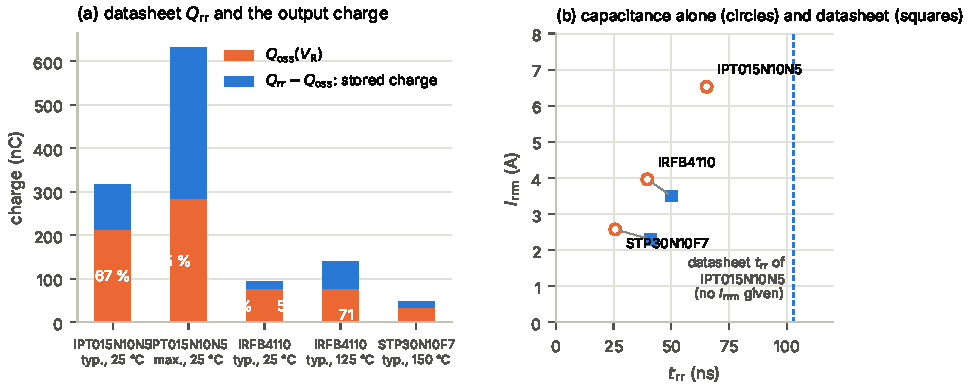
\includegraphics[width=\textwidth]{figures/fig_floor.pdf}
\caption{(a) The datasheet $\Qrr$ of the three devices and the part of it that is the output charge $\Qoss(\VR)$ (the percentage); the rest is stored charge. (b) The recovery that the output capacitance alone would produce in the test, \eqref{eq:floor} (circles), against the peak current and recovery time printed in the datasheets (squares); for \IPT{} only the recovery time is given.}
\label{fig:floor}
\end{figure}

\subsection{The capacitance alone}
\label{sec:floor}
Suppose the device stores no charge at all. The junction blocks at the current zero, the driver goes on pulling current along the ramp, and that current charges $\Coss$: $\Coss\,\diff v/\diff t = a\,t$ from the current zero. The voltage reaches $\VR$ when $a t^2/2 = \Qoss(\VR)$, the current drops, and the test prints
\begin{equation}
\Irrm = \sqrt{2a\,\Qoss(\VR)} , \qquad \trr = \sqrt{\frac{2\Qoss(\VR)}{a}} , \qquad \Qrr = \Qoss(\VR) .
\label{eq:floor}
\end{equation}
This is the \emph{capacitive floor}: the smallest recovery a MOSFET can show in the test, with nothing to do with stored charge. At \SI{100}{\ampere\per\micro\second} it is \SI{\bdIptCapIrrm}{\ampere}, \SI{\bdIptCapTrr}{\nano\second} and \SI{\bdIptQoss}{\nano\coulomb} for \IPT{}, \SI{\bdIrfCapIrrm}{\ampere}, \SI{\bdIrfCapTrr}{\nano\second} and \SI{\bdIrfQoss}{\nano\coulomb} for \IRF{}, \SI{\bdStpCapIrrm}{\ampere}, \SI{\bdStpCapTrr}{\nano\second} and \SI{\bdStpQoss}{\nano\coulomb} for \STP{} (Fig.~\ref{fig:floor}b). For \IRF{} at \SI{25}{\celsius} the datasheet prints \SI{\bdIrfIrrm}{\ampere}, \SI{\bdIrfLoTrr}{\nano\second} and \SI{\bdIrfLoQrr}{\nano\coulomb}: the floor itself, within the tolerance of typical values. For \STP{} at \SI{150}{\celsius} the datasheet peak of \SI{\bdStpIrrm}{\ampere} is below the floor of \SI{\bdStpCapIrrm}{\ampere} that the estimated output charge gives. In both cases the triangle $\Irrm^2/(2a)$ of the datasheet peak (\SI{\bdIrfTri}{\nano\coulomb} and \SI{\bdStpTri}{\nano\coulomb}) is larger than the stored charge of \eqref{eq:qdifds} (\SI{\bdIrfLoQdif}{\nano\coulomb} and \SI{\bdStpQdif}{\nano\coulomb}): the three typical values are not consistent with each other and with the capacitance, and no parameter set can return all three. What they say is that the stored charge of these two devices is at or below the resolution of their datasheets, and that the peak they print is the capacitive current.

\subsection{What the terminals show during the voltage rise}
\label{sec:terminals}
After the junction blocks, the diffusion current is a source that decays, $\idif = -\Irr\,e^{-(t-\Tone)/\taurr}$, and the voltage rises at the rate at which the driver supplies current beyond it: $\Coss(v)\,\diff v/\diff t = |i| - |\idif|$. The driver is a MOSFET turning on with an inductive load, and two idealisations bound what its current does once the voltage of the device under test starts to move.
\begin{itemize}
\item \emph{Driver that keeps the slope.} The gate of the driver goes on charging and its current goes on rising at the rate $a$. The terminal current of the device under test follows the ramp past the diffusion peak, the capacitive current being the difference, until the voltage reaches $\VR$ at $\Ttwo$. The terminal peak is $\Irrm = a\,(\Ttwo - t_0)$, with $\Ttwo$ from
\begin{equation}
\frac{a}{2}\bigl[(\Ttwo - t_0)^2 - \ta^2\bigr] - \Irr\,\taurr\bigl(1 - e^{-\Tc/\taurr}\bigr) = \Qoss(\VR) , \qquad \Tc = \Ttwo - \Tone .
\label{eq:rampdriver}
\end{equation}
The capacitive floor \eqref{eq:floor} is this limit with $\Irr \to 0$.
\item \emph{Driver held at the Miller plateau.} When the voltage of the device under test starts to rise, the drain voltage of the driver falls, its gate current goes into its own $\Cgd$, and its channel current stays where it was: at $\IF + \Irr$. The terminal current of the device under test then stays at $\Irr$, a flat top, and the voltage rises only as fast as the decaying diffusion current frees current for the capacitance. The flat top lasts $\Tc$, from
\begin{equation}
\Irr\,\Tc - \Irr\,\taurr\bigl(1 - e^{-\Tc/\taurr}\bigr) = \Qoss(\VR) ,
\label{eq:plateaudriver}
\end{equation}
and the terminal peak is the diffusion peak, $\Irrm = \Irr$.
\end{itemize}
A real driver is in between: its gate goes on charging at some rate, and the rate at which the voltage of the device under test can rise is limited by the current the driver makes available, which the datasheet does not state. In both limits, when the voltage reaches $\VR$ the terminal current drops in a step to the diffusion current left, $\Irr e^{-\Tc/\taurr}$, which is small when $\Tc$ is several $\taurr$; so the fall of the current is a step at $\Ttwo$, the recovery time is $\Ttwo - t_0$ for every convention of Sec.~\ref{sec:model}, and the charge to the end of the recovery is $\Qdif + \Qoss(\VR)$ plus the small terms of Sec.~\ref{sec:balance}. The output capacitance makes the body diode look snappy whatever its softness: the recovery ends when the capacitance is charged, not when the tail is over.

Table~\ref{tab:drivers} summarises what the two limits print. The charge is the same; the peak current differs by the capacitive current, which for \IPT{} is twice the diffusion peak; the recovery time differs because the capacitance charges faster when the driver pushes.

\begin{table}[htb]
\centering\small
\caption{The recovery test at the terminals in the two driver limits, for a device with the stored-charge recovery $\Irr$, $\taurr$ and the output charge $\Qoss(\VR)$.}
\label{tab:drivers}
\setlength{\tabcolsep}{5pt}
\begin{tabular}{@{}lccc@{}}
\toprule
 & Driver that keeps the slope & Driver at the Miller plateau & Capacitance alone \\
\midrule
Terminal peak $\Irrm$ & $a\,(\Ttwo - t_0) > \Irr$, \eqref{eq:rampdriver} & $\Irr$ & $\sqrt{2a\Qoss(\VR)}$ \\
Recovery time $\trr$ & $\Irrm/a$ & $\ta + \Tc$, \eqref{eq:plateaudriver} & $\sqrt{2\Qoss(\VR)/a}$ \\
Charge $\Qrr$ & $\Qdif + \Qoss(\VR)$ & $\Qdif + \Qoss(\VR)$ & $\Qoss(\VR)$ \\
Fall of the current & step & step & step \\
\IPT{} with the set of Table~\ref{tab:sets} & \SI{\bdIptRefRIrrm}{\ampere}, \SI{\bdIptRefRTrr}{\nano\second} & \SI{\bdIptRefIrrm}{\ampere}, \SI{\bdIptRefTrr}{\nano\second} & \SI{\bdIptCapIrrm}{\ampere}, \SI{\bdIptCapTrr}{\nano\second} \\
\bottomrule
\end{tabular}
\end{table}

\subsection{The output charge from the datasheet}
\label{sec:qoss}
Four cases, in decreasing order of what the datasheet gives.
\begin{enumerate}
\item \emph{$\Qoss$ printed.} Infineon prints the output charge at $V_\mathrm{DD} = \SI{50}{\volt}$, which is also the $\VR$ of its recovery test: $\Qoss(\VR)$ is read directly. If the two voltages differ, the charge is moved with the power law below.
\item \emph{Effective capacitance.} The IRF datasheet prints $C_\mathrm{oss(tr)}$ over \SIrange{0}{80}{\volt}, defined so that $\Qoss(\SI{80}{\volt}) = C_\mathrm{oss(tr)}\cdot\SI{80}{\volt} = \SI{\bdIrfQossEighty}{\nano\coulomb}$; the recovery test is at \SI{85}{\volt}, and the law below gives \SI{\bdIrfQoss}{\nano\coulomb}. (The energy-related $C_\mathrm{oss(er)}$ does not give the charge.)
\item \emph{The curve.} With the curve $\Coss(\VDS)$ read at a few voltages, the integral is a trapezoidal sum, or the power law is fitted to the points.
\item \emph{One capacitance.} With $\Coss$ at \SI{50}{\volt} only, as for \STP{}, the shape has to be assumed; the estimate of Fig.~\ref{fig:floor} uses $m = \bdStpMassumed$, the exponent of an abrupt junction, and is uncertain by tens of percent.
\end{enumerate}
The power law used for the simulations and for moving a charge from one voltage to another is the depletion law of a junction,
\begin{equation}
\Coss(v) = \frac{\Czero}{(1 + v/\Vj)^m} , \qquad \Qoss(V) = \frac{\Czero\Vj}{1-m}\Bigl[\Bigl(1+\frac{V}{\Vj}\Bigr)^{1-m} - 1\Bigr] ,
\label{eq:cosslaw}
\end{equation}
with the potential $\Vj$ chosen and $\Czero$, $m$ fitted to two data: for \IPT{}, $\Coss(\SI{50}{\volt}) = \SI{\bdIptCoss}{\pico\farad}$ and $\Qoss(\SI{50}{\volt}) = \SI{\bdIptQoss}{\nano\coulomb}$ give, with $\Vj = \SI{\bdIptVj}{\volt}$, $\Czero = \SI{\bdIptCzero}{\nano\farad}$ and $m = \bdIptM$ (Fig.~\ref{fig:coss}). The potential sets how the capacitance behaves below a few volts, which the two data do not fix; Sec.~\ref{sec:simulated} shows that it moves the extracted parameters little. The exponent is larger than the 0.5 of an abrupt junction because the real curve of a trench MOSFET is steeper: the depletion reaches the trench bottoms and the capacitance falls faster than the junction law in the tens of volts.

\begin{figure}[htb]
\centering
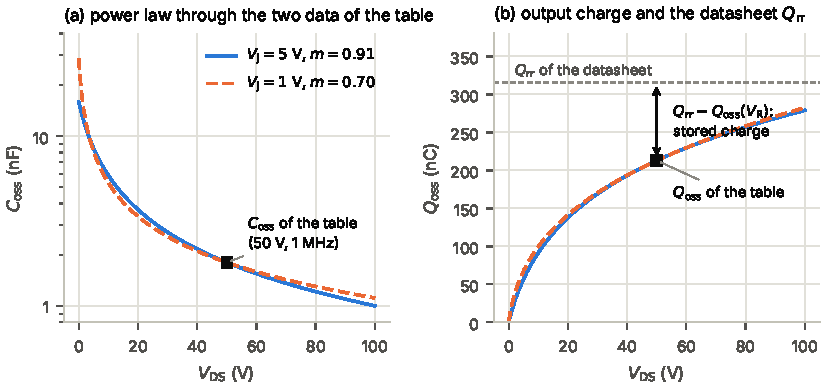
\includegraphics[width=\textwidth]{figures/fig_coss.pdf}
\caption{\IPT{}: (a) output capacitance by the power law \eqref{eq:cosslaw} through the two data of the table, for two choices of the potential $\Vj$; (b) the output charge, with the datasheet $\Qoss$ and $\Qrr$ at \SI{50}{\volt}: the stored charge is the gap between the two.}
\label{fig:coss}
\end{figure}

%=====================================================================
\section{From the datasheet to the parameters}
\label{sec:extraction}
\subsection{The stored charge}
Step one is \eqref{eq:qdifds}: $\Qdif = \Qrr - \Qoss(\VR)$, with the output charge of Sec.~\ref{sec:qoss} at the voltage of the test. If the difference is small against $\Qrr$ or negative, the stored charge is below the resolution of the data: the body diode is modelled as the capacitance plus a small charge (a set with the capacitive-floor shape, or a set scaled from a hotter test point by the area), and the datasheet values are not converted as if they were a diode.

\subsection{The second datum}
\label{sec:second}
The recovery has two parameters, so a second datum is needed, and the datasheet gives it at the terminals. Three cases.
\begin{itemize}
\item \emph{Recovery time given, no peak} (Infineon, Table~\ref{tab:data}). Under the plateau limit $\trr = \ta + \Tc$ with $\Tc$ from \eqref{eq:plateaudriver}, and $\Qdif = \Irr^2/(2a) + \Irr\taurr$: two equations in $\Irr$ and $\taurr$, solved by a one-dimensional search on $\Irr$ (\texttt{invert\_terminal} in the scripts). Under the slope-keeping limit $\trr = \Irrm/a$ and $\Irrm^2/(2a) \leq \Qrr$ is required; for \IPT{} that would need a terminal triangle of \SI{\bdIptRampTri}{\nano\coulomb} against a $\Qrr$ of \SI{\bdIptQrr}{\nano\coulomb}, so the data are consistent with the plateau limit only, and that is what is used.
\item \emph{Peak given} (IRF, ST). Under the plateau limit $\Irr = \Irrm$ directly, and \eqref{eq:taurr} with $\Qdif$ gives $\taurr$; it needs $\Irrm^2/(2a) < \Qdif$. Under the slope-keeping limit $\Irr < \Irrm$ is found from \eqref{eq:rampdriver}. For the two datasheets with a peak the condition fails under both limits (Sec.~\ref{sec:floor}).
\item \emph{Neither consistent, or charge alone.} The softness is assumed and \eqref{eq:fromq} used. The lifetime depends little on it (Fig.~\ref{fig:bracket}a); the transit time is then a guess, to be bracketed in the simulation.
\end{itemize}
The recovery time at the terminals does not depend on the convention of its definition, because the fall is a step (Sec.~\ref{sec:terminals}): for \IPT{} the straight-line, \SI{25}{\percent} and \SI{10}{\percent} conventions give sets that differ by \SI{\bdIptConvSpread}{\percent}. This is one convention less to worry about than for a discrete diode.

\subsection{Lifetime and transit time}
With $\Irr$ and $\taurr$ of the stored charge, \eqref{eq:iter} and \eqref{eq:tm} give $\tau$ and $\TM$. On the long ramp of the test the iteration stops at its first step: $\tau = \taurr + \Irr/a$, $\TM = \tau\taurr a/\Irr$. The plausibility check of Sec.~\ref{sec:thinbase} then reads: $\tau$ of the order of $W^2/(2D)$ and $\TM = \tau s/2$ with a softness below one for a thin base.

\subsection{Conduction, blocking, capacitance for the simulator}
\label{sec:static}
\emph{Forward characteristic.} The datasheet gives one point, $\VSD$ at a current, and a curve. With one point two of the three parameters $\IS$, $n$, $\RS$ have to be chosen. The base is in high injection at the rated current of a low-voltage MOSFET (a current density of hundreds of amperes per square centimetre in a drift region doped around $10^{16}\,\si{\per\centi\metre\cubed}$), so $n = 2$ as for a power diode; $\RS$ is the resistance of substrate, metal and package, a fraction of $\Rds$ (the drift region is conductivity modulated). Then $\IS = I/[e^{(\VSD - \RS I)/(n\VT)} - 1]$. With the curve, three points fix all three \cite{lmnote}. An implementation that writes the junction law as $\tau\IS^{*}(e^{\vj/(n\VT)}-1)$, such as the library component \texttt{diode\_rr} and \texttt{mos\_dyn}, needs $\IS^{*} = \IS(\tau+\TM)/\tau$.

\emph{Leakage.} $\Rr = \VDS/I_\mathrm{DSS}$ at the temperature of interest; it does not matter for the recovery.

\emph{Capacitance.} In a simulation where the body diode is a Lauritzen--Ma diode in parallel with an ideal switch, the junction capacitance of the diode is $\Coss(v)$ of \eqref{eq:cosslaw}. In a MOSFET model that has its own $\Cgd$ and $\Cds$, such as \texttt{mos\_dyn}, the diode carries only the diffusion charge and $\Cds = \Coss - \Crss$ is the drain-source capacitance of the model; the comment at the top of \texttt{mos\_dyn.ssc} says so. In both cases the recovery parameters are the ones converted from the stored charge: the capacitance is in the circuit, and must not be in $\tau$ and $\TM$ as well.

\subsection{The error of not subtracting the output charge}
\label{sec:naive}
The fitting hints of \texttt{mos\_dyn.ssc} \cite{mosdyn} convert $\Qrr$ and $\Irr$ of the datasheet with the long-ramp closed forms as they are. For a MOSFET that double-counts the output charge, which the component also has as $\Cds$. For \IPT{}, converting the datasheet $\Qrr$ and $\trr$ as a diode with the \SI{25}{\percent} convention gives $\Irr = \SI{\bdIptNIrr}{\ampere}$, $\tau = \SI{\bdIptNTau}{\nano\second}$ and $\TM = \SI{\bdIptNTm}{\nano\second}$ (with the equal-charge convention $\tau = \SI{\bdIptNTriTau}{\nano\second}$, $\TM = \SI{\bdIptNTriTm}{\nano\second}$), against $\tau = \SI{\bdIptRefTau}{\nano\second}$ and $\TM = \SI{\bdIptRefTm}{\nano\second}$: the lifetime is doubled and the transit time is five times too long. In the simulated test with $\Coss$ in parallel this set returns $\Qrr = \SI{\bdIptNSimQrr}{\nano\coulomb}$, \SI{\bdIptNSimQrrErr}{\percent} above the datasheet (Fig.~\ref{fig:test}a, dotted), and in a converter it would charge the turn-on of the opposite switch with the output charge twice.

%=====================================================================
\section{Worked example: \IPT{}}
\label{sec:example}
\subsection{Closed forms}
\label{sec:closed}
The data are the first column of Table~\ref{tab:data}: $\IF = \SI{\bdIptIf}{\ampere}$, $a = \SI{\bdIptSlope}{\ampere\per\micro\second}$, $\VR = \SI{\bdIptVr}{\volt}$, $\Qrr = \SI{\bdIptQrr}{\nano\coulomb}$, $\trr = \SI{\bdIptTrr}{\nano\second}$, $\Qoss(\SI{50}{\volt}) = \SI{\bdIptQoss}{\nano\coulomb}$, all typical values at \SI{25}{\celsius}.
\begin{enumerate}
\item \emph{Stored charge.} $\Qdif = \Qrr - \Qoss(\VR) = \bdIptQrr - \bdIptQoss = \SI{\bdIptQdif}{\nano\coulomb}$, \SI{\bdIptQdifPct}{\percent} of the datasheet charge.
\item \emph{Second datum.} The recovery time under the plateau limit: $\ta + \Tc = \trr$ with $\Tc$ from \eqref{eq:plateaudriver}, and $\Irr^2/(2a) + \Irr\taurr = \Qdif$. The search on $\Irr$ gives $\Irr = \SI{\bdIptIrr}{\ampere}$, $\ta = \SI{\bdIptTa}{\nano\second}$, $\taurr = \SI{\bdIptTaurr}{\nano\second}$ and a flat top of $\Tc = \SI{\bdIptTc}{\nano\second}$; the triangle holds \SI{\bdIptQtri}{\nano\coulomb} and the tail \SI{\bdIptQtail}{\nano\coulomb}. At the end of the flat top the diffusion current left is $\Irr e^{-\Tc/\taurr}$, a few milliamperes: the current falls in a step. Under the slope-keeping limit there is no solution (Sec.~\ref{sec:second}).
\item \emph{Lifetime and transit time.} The ramp lasts $\Tone/\tau \approx \bdIptX$ lifetimes, so the first step of the iteration \eqref{eq:iter} is the answer: $\tau = \taurr + \Irr/a = \SI{\bdIptTauOne}{\nano\second}$, $\TM = \tau\taurr a/\Irr = \SI{\bdIptTmOne}{\nano\second}$ (the iteration stops after \bdIptIter{} steps without changing them). Softness $s = 2\taurr/\ta = \bdIptS$, $\rho = \taurr/\tau = \bdIptRho$.
\item \emph{Plausibility.} The diffusion length $\sqrt{D\tau}$ of the bulk would be \SI{\bdIptLdiff}{\micro\metre}, about the width of the drift region: the base does not recombine, it stores, and $\tau$ is a storage time. Read as $W^2/(2D)$ it corresponds to $W = \SI{\bdIptWstore}{\micro\metre}$, at the top of the range of a \SI{100}{\volt} drift region; read through $\TM = d^2/(3D)$ with the lumped profile of \cite{lmnote} it corresponds to a base of \SI{\bdIptWpar}{\micro\metre}. Both are the right size for the device [M], and that is all the check can say.
\item \emph{Static parameters.} With $n = \bdIptN$ and $\RS = \SI{\bdIptRs}{\milli\ohm}$: $\IS = \bdIptIsTwo$~A from $\VSD = \SI{\bdIptVsd}{\volt}$ at \SI{\bdIptIvsd}{\ampere}, $\IS^{*} = \bdIptIsStarTwo$~A for an implementation that uses $\IS^{*}$; the model then gives \SI{\bdIptVtenTwo}{\volt} at \SI{10}{\ampere} and \SI{\bdIptVthreeTwo}{\volt} at \SI{300}{\ampere}. With $n = 1$: $\IS = \bdIptIsOne$~A, \SI{\bdIptVtenOne}{\volt} and \SI{\bdIptVthreeOne}{\volt}; the datasheet curve decides between the two. $\Rr = \SI{\bdIptRr}{\mega\ohm}$ at \SI{25}{\celsius} for a leakage of \SI{1}{\micro\ampere}, \SI{\bdIptRrHot}{\mega\ohm} at \SI{125}{\celsius}. Capacitance: the power law of Fig.~\ref{fig:coss}.
\end{enumerate}

\subsection{The simulated test}
\label{sec:simulated}
The closed forms treat the recovery as the sum of two ideal pieces: the diffusion current of the model with the current imposed, and a capacitance that charges after the junction blocks. The check is a simulation of the test with the complete device: the two-charge model with the forward characteristic of step~5, the capacitance $\Coss(v)$ of \eqref{eq:cosslaw} across the junction, the leakage, and the circuit of Fig.~\ref{fig:testcircuit} in three phases (\texttt{simulate\_test} in \texttt{body\_diode\_lm.py}). In the first the driver imposes the ramp $\IF - at$ on the terminals and the junction voltage is a state variable: the capacitance takes current as soon as the junction voltage moves, well before it reverses. The phase ends when the junction voltage crosses zero, which is the event that defines $\Tone$ here. In the second the driver either keeps its slope or holds its current, and the voltage rises until it reaches $\VR$. In the third the device sits across the source $\VR$ through a stray inductance $\Ls = \SI{\bdIptLs}{\nano\henry}$ and a damping resistance $\Rser = \SI{\bdIptRser}{\ohm}$, and the current rings back to zero. The charge is integrated from the current zero to the first return of the current to zero after the peak, as a datasheet does, and the recovery time is read at \SI{25}{\percent} of the peak (the straight-line convention gives the same number within a nanosecond, as Sec.~\ref{sec:terminals} says it must).

With the set of the closed forms the simulated test returns, under the plateau driver, $\Irrm = \SI{\bdIptSimPIrrm}{\ampere}$, $\Qrr = \SI{\bdIptSimPQrr}{\nano\coulomb}$ (\SI{\bdIptSimPQrrErr}{\percent}) and $\trr = \SI{\bdIptSimPTrr}{\nano\second}$ (\SI{\bdIptSimPTrrErr}{\percent}): close, and the difference has two identifiable causes. The junction blocks \SI{\bdIptSimPTone}{\nano\second} after the current zero instead of the \SI{\bdIptTa}{\nano\second} of the closed form, because while the junction voltage falls from its forward value (\SI{\bdIptVjzero}{\volt}) to zero the capacitance, largest there, releases about \SI{\bdIptSimQfwd}{\nano\coulomb} and the diffusion current is by that much below the ramp; and the voltage overshoots $\VR$ to \SI{\bdIptSimPVpk}{\volt} on the stray inductance, which is another \SI{\bdIptSimQover}{\nano\coulomb} of capacitive charge counted in $\Qrr$. Both are properties of the test, not of the stored charge, and both are in a real measurement too.

The set is then refined on the simulated test: $\tau$ and $\TM$ are adjusted until the simulation returns the datasheet $\Qrr$ and $\trr$ (a least-squares fit in the logarithms, \bdIptRefNsim{} simulations). The result is $\tau = \SI{\bdIptRefTau}{\nano\second}$ (\SI{\bdIptRefTauErr}{\percent} against the closed form) and $\TM = \SI{\bdIptRefTm}{\nano\second}$ (\SI{\bdIptRefTmErr}{\percent}), with a peak of \SI{\bdIptRefIrrm}{\ampere}, Fig.~\ref{fig:test}a. Repeating the refinement with the steeper capacitance law of Fig.~\ref{fig:coss} ($\Vj = \SI{1}{\volt}$, $\Czero = \SI{\bdIptAltCzero}{\nano\farad}$, $m = \bdIptAltM$) gives $\tau = \SI{\bdIptAltTau}{\nano\second}$ and $\TM = \SI{\bdIptAltTm}{\nano\second}$: the shape of the capacitance at low voltage, which the datasheet does not fix, moves the lifetime by a few percent and the transit time by half. This is the pattern of the whole of Table~\ref{tab:sets}: whatever is uncertain in the data or in the driver lands on $\TM$, while $\tau$ is set by the stored charge and the slope alone, $\tau \approx \sqrt{2\Qdif/a}$ up to the softness.

Figure~\ref{fig:test}b shows the same device, with the refined set, in a test whose driver keeps its slope: the terminal peak is \SI{\bdIptRefRIrrm}{\ampere} instead of \SI{\bdIptRefIrrm}{\ampere}, the recovery time \SI{\bdIptRefRTrr}{\nano\second} instead of \SI{\bdIptRefTrr}{\nano\second}, the charge \SI{\bdIptRefRQrr}{\nano\coulomb} instead of \SI{\bdIptRefQrr}{\nano\coulomb}. Two laboratories with the same device and the same nominal $\IF$, $a$ and $\VR$ would print these two triples, and only the charge agrees. The dotted trace of Fig.~\ref{fig:test}a is the set converted without subtracting the output charge (Sec.~\ref{sec:naive}): \SI{\bdIptNSimQrr}{\nano\coulomb}, a recovery time of \SI{\bdIptNSimTrr}{\nano\second}, and a tail that goes on after the voltage has reached $\VR$ because its transit time is five times too long. The last row of the table is the capacitance alone, with $\tau$ set to a fraction of a nanosecond: the simulation returns \SI{\bdIptCapSimIrrm}{\ampere} against the \SI{\bdIptCapIrrm}{\ampere} of \eqref{eq:floor}, and a charge of \SI{\bdIptCapSimQrr}{\nano\coulomb} that exceeds $\Qoss(\VR)$ by the two contributions of the test described above.

\begin{figure}[htb]
\centering
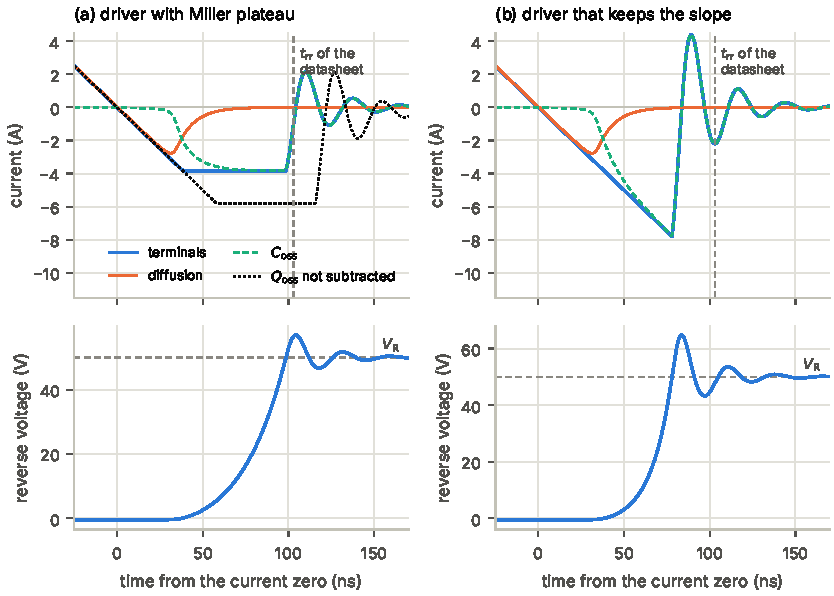
\includegraphics[width=\textwidth]{figures/fig_test.pdf}
\caption{\IPT{}, simulated recovery test with the refined set of Table~\ref{tab:sets} ($\IF = \SI{\bdIptIf}{\ampere}$, $a = \SI{\bdIptSlope}{\ampere\per\micro\second}$, $\VR = \SI{\bdIptVr}{\volt}$): terminal current, its diffusion and capacitive parts, and the voltage. (a) Driver held at the Miller plateau: flat top at the diffusion peak while the capacitance charges, step when the voltage reaches $\VR$, ringing on the stray inductance. Dotted: the set converted without subtracting $\Qoss(\VR)$. (b) Driver that keeps the slope: the terminal current follows the ramp past the diffusion peak.}
\label{fig:test}
\end{figure}

\begin{table}[htb]
\centering\small
\caption{\IPT{}: parameter sets, and what the simulated test with the plateau driver returns with each. Datasheet: $\Qrr = \SI{\bdIptQrr}{\nano\coulomb}$, $\trr = \SI{\bdIptTrr}{\nano\second}$, no peak given.}
\label{tab:sets}
\setlength{\tabcolsep}{4pt}
\begin{tabular}{@{}lccc>{\raggedright\arraybackslash}p{5.2cm}ccc@{}}
\toprule
Set & $\tau$ (ns) & $\TM$ (ns) & $s$ & How obtained & $\Irrm$ (A) & $\Qrr$ (nC) & $\trr$ (ns) \\
\midrule
Closed forms & \bdIptTau & \bdIptTm & \bdIptS & $\Qrr - \Qoss(\VR)$ and $\trr$, plateau limit (Sec.~\ref{sec:closed}) & \bdIptSimPIrrm & \bdIptSimPQrr & \bdIptSimPTrr \\
\textbf{Refined} & \textbf{\bdIptRefTau} & \textbf{\bdIptRefTm} & \bdIptRefS & simulated test fitted to $\Qrr$ and $\trr$ & \bdIptRefIrrm & \bdIptRefQrr & \bdIptRefTrr \\
Refined, steep $\Coss$ law & \bdIptAltTau & \bdIptAltTm & -- & as above, with $\Vj = \SI{1}{\volt}$ & -- & -- & -- \\
Charge alone, $s = 0.25$ & \bdIptSQuarterTau & \bdIptSQuarterTm & 0.25 & \eqref{eq:fromq}, softness assumed & \bdIptSQuarterIrr$^{\dagger}$ & -- & \bdIptSQuarterTrrP$^{\dagger}$ \\
Charge alone, $s = 2$ & \bdIptSTwoTau & \bdIptSTwoTm & 2 & \eqref{eq:fromq}, softness assumed & \bdIptSTwoIrr$^{\dagger}$ & -- & \bdIptSTwoTrrP$^{\dagger}$ \\
$\Qoss$ not subtracted & \bdIptNTau & \bdIptNTm & -- & $\Qrr$, $\trr$ converted as a diode (\SI{25}{\percent} convention) & \bdIptNSimIrrm & \bdIptNSimQrr & \bdIptNSimTrr \\
Maximum values & \bdIptXTau & \bdIptXTm & \bdIptXS & maxima of $\Qrr$, $\trr$, $\Qoss$, Sec.~\ref{sec:maxima} & -- & -- & -- \\
Capacitance alone & $\to 0$ & -- & -- & \eqref{eq:floor} gives \bdIptCapIrrm~A, \bdIptQoss~nC, \bdIptCapTrr~ns & \bdIptCapSimIrrm$^{\ddagger}$ & \bdIptCapSimQrr$^{\ddagger}$ & \bdIptCapSimTrr$^{\ddagger}$ \\
\bottomrule
\end{tabular}
\\[3pt]
\begin{minipage}{0.95\textwidth}\footnotesize
$^{\dagger}$ closed forms of the plateau limit, not simulated. $^{\ddagger}$ simulated with the driver that keeps the slope: with no stored charge the plateau limit has no flat top, because the driver current at the blocking instant is zero.
\end{minipage}
\end{table}

\subsection{When only the charge is usable}
\label{sec:bracket}
If the datasheet gives no recovery time, or gives one that no driver model can reconcile with the charge (the two other devices, Sec.~\ref{sec:others}), the second datum is an assumed softness and \eqref{eq:fromq} gives the set. Figure~\ref{fig:bracket}a shows what \IPT{} would get for a softness anywhere from 0.1 to 2.5: the lifetime stays within \SIrange{\bdIptSQuarterTau}{\bdIptSTwoTau}{\nano\second} for $s$ from 0.25 to 2, because on a long ramp $\Qdif = a(\tau^2 - \taurr^2)/2$ and $\taurr \ll \tau$ for any plausible softness; the transit time runs from \SI{\bdIptSQuarterTm}{\nano\second} to \SI{\bdIptSTwoTm}{\nano\second}, because $\TM = \tau s/2$ \emph{is} the softness. Figure~\ref{fig:bracket}b shows what the test would print for each of these sets: under the plateau driver the recovery time grows with the softness, from \SI{\bdIptSQuarterTrrP}{\nano\second} to \SI{\bdIptSTwoTrrP}{\nano\second}, and the datasheet value selects $s = \bdIptS$; under a driver that keeps its slope it is \SI{\bdIptSQuarterTrrR}{\nano\second} whatever the softness, because then $\trr = \Irrm/a$ and the terminal peak is set almost entirely by the charge. This is the second reason why the stored charge is the robust datum and the recovery time is not: the time tells about the driver as much as about the diode.

For a thin-base body diode without lifetime control the softness found here is $\bdIptS$, and for the two other devices \num{\bdIrfHiS} and \num{\bdStpS} (Sec.~\ref{sec:others}); a value between 0.25 and 0.5 is the assumption to make when the data give nothing better. The transit time it produces is a guess that the simulation of the application should bracket: it sets how fast the current snaps back once the capacitance is charged, and in a converter this is mostly the ringing with the stray inductance.

\begin{figure}[htb]
\centering
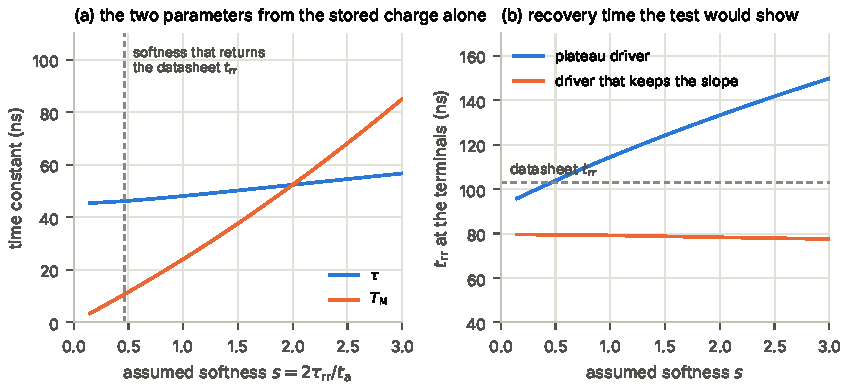
\includegraphics[width=\textwidth]{figures/fig_bracket.pdf}
\caption{\IPT{}, the set from the stored charge $\Qrr - \Qoss(\VR)$ and an assumed softness. (a) Lifetime and transit time against the softness: $\tau$ barely moves, $\TM$ is the softness. (b) The recovery time the test would show with each set, in the two driver limits; the datasheet value selects the softness under the plateau limit, and gives no information under the other.}
\label{fig:bracket}
\end{figure}

\subsection{Maximum values}
\label{sec:maxima}
Infineon prints maxima at twice the typical values: $\Qrr = \SI{\bdIptQrrMax}{\nano\coulomb}$, $\trr = \SI{\bdIptTrrMax}{\nano\second}$, and $\Qoss = \SI{\bdIptQossMax}{\nano\coulomb}$. Converted as a set they give $\Qdif = \SI{\bdIptQdifMax}{\nano\coulomb}$, $\Irr = \SI{\bdIptXIrr}{\ampere}$, $\tau = \SI{\bdIptXTau}{\nano\second}$, $\TM = \SI{\bdIptXTm}{\nano\second}$ and a softness of \num{\bdIptXS}: a transit time three times the lifetime, which no thin base has. The maxima are guard bands applied at the same time to quantities that do not move together, and a set made of them describes no device. For a worst case the typical set is scaled instead: keeping the softness, the stored charge recovered on a long ramp goes as $\tau^2$, so a stored charge of \SI{\bdIptQdifMax}{\nano\coulomb} corresponds to $\tau$ and $\TM$ multiplied by $\sqrt{\bdIptQdifMax/\bdIptQdif} = \bdIptXScale$. The recovery time that the test would show grows by less than that, because the flat top $\Tc \approx \Qoss(\VR)/\Irr$ shrinks as the peak grows.

%=====================================================================
\section{The channel in parallel}
\label{sec:channel}
\subsection{With the channel on, nothing is stored}
\label{sec:channelon}
In synchronous rectification the third-quadrant current flows through the channel for most of the conduction time, and the body diode sees only the drop of the channel, $\Rds\,I$. For \IPT{} at \SI{100}{\ampere} that is \SI{\bdIptChVHundred}{\milli\volt}; with the forward parameters of Sec.~\ref{sec:closed} the diode carries $\bdIptChIHundred$~A and stores $\bdIptChQHundred$~C, which is nothing. At \SI{300}{\ampere}, \SI{\bdIptChVThree}{\milli\volt} across the junction, the diode current is $\bdIptChIThree$~A and the stored charge $\bdIptChQThree$~C, still a thousandth of what the diode alone would store. The exponential of the junction makes the division sharp: below about half a volt the channel carries everything and the base is empty. So the charge that recovers at a commutation is the charge stored during the dead time only, and the recovery of a synchronous rectifier is set by the dead time, not by the conduction time. In a simulation this comes by itself from a diode model in parallel with the channel resistance, provided the diode has the exponential junction law with a sensible $\IS$ and $n$: a piecewise-linear diode with a threshold would decide, wrongly, how the current splits.

\subsection{The dead time}
\label{sec:deadtime}
When the channel turns off at the start of the dead time the current moves to the body diode within the switching time of the gate, and the base fills from empty with the time constant $\tau$: $\qM(t) = \tau\IF(1 - e^{-t/\tau})$, that is \SI{\bdAppFillTwenty}{\percent} of the steady charge after \SI{\bdAppTdTwenty}{\nano\second}, \SI{\bdAppFillFifty}{\percent} after \SI{\bdAppTdFifty}{\nano\second} and \SI{\bdAppFillHundred}{\percent} after \SI{\bdAppTdHundred}{\nano\second} for $\tau = \SI{\bdAppTau}{\nano\second}$. A dead time of a few tens of nanoseconds, usual in a low-voltage leg, is of the order of the lifetime, and the question is how much less the diode recovers when the ramp starts from a base that is not full. Appendix~\ref{app:deadtime} solves the ramp from an arbitrary initial charge: the diffusion current is still the imposed ramp until the junction blocks, so the recovery is still a triangle of height $\Irr$ plus a tail $\Irr\taurr$, and only the blocking instant moves. The result depends on one number, $\lambda = \IF/(a\tau)$, the duration of the ramp in lifetimes (Fig.~\ref{fig:deadtime}a): when the ramp is long, $\lambda \gg 1$, the base reaches its steady state during the ramp whatever it held at the start, and the dead time has no effect; when the ramp is short, the charge at the start of the ramp is what is recovered, and the dead time matters. At the datasheet slope $\lambda = \bdAppLamDs$, and a dead time of \SI{20}{\nano\second} changes the recovered charge by nothing (\SI{\bdAppQdsTdTwenty}{\nano\coulomb} either way). At the slopes of a \SI{48}{\volt} leg the ramp is short: at \SI{\bdAppTwoSlope}{\ampere\per\nano\second} $\lambda = \bdAppTwoLam$, and a dead time of \SI{20}{\nano\second} leaves \SI{\bdAppTwoTwentyQPct}{\percent} of the steady-state recovered charge, one of \SI{50}{\nano\second} \SI{\bdAppTwoFiftyQPct}{\percent} (Fig.~\ref{fig:deadtime}b and Table~\ref{tab:app}). The dead time is a second-order lever on the recovery of a low-voltage MOSFET, and only on fast ramps; the first-order lever is the slope, Sec.~\ref{sec:slope}.

\begin{figure}[htb]
\centering
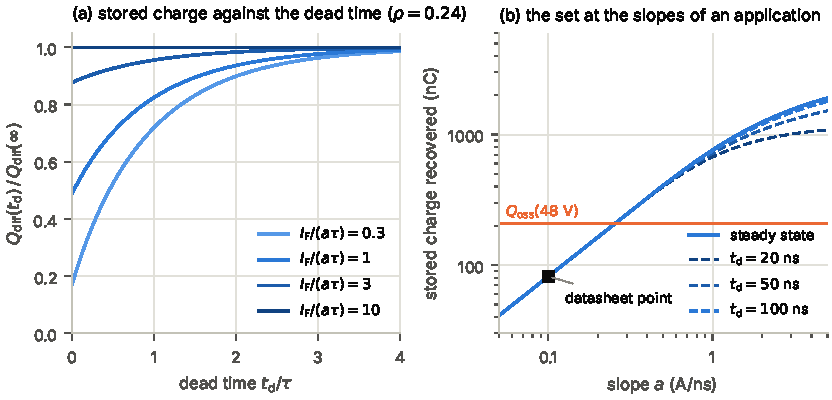
\includegraphics[width=\textwidth]{figures/fig_deadtime.pdf}
\caption{\IPT{}, refined set. (a) Stored charge recovered after a dead time $\td$, relative to the steady state, for ramps of different length $\lambda = \IF/(a\tau)$: a long ramp forgets the initial state. (b) Stored charge recovered against the slope of the commutation, from a full base and after three dead times, with the output charge at \SI{48}{\volt} for comparison; the datasheet slope is at the left edge.}
\label{fig:deadtime}
\end{figure}

\subsection{Connecting the model in a simulator}
\label{sec:connect}
Two arrangements are in use, and the capacitance must be in one place only.
\begin{itemize}
\item \emph{Switch plus diode.} The MOSFET is an ideal or resistive switch with no capacitance of its own, and the body diode is a Lauritzen--Ma diode in anti-parallel: the \emph{Diode with Reverse Recovery} of PLECS \cite{plecs}, the \emph{Diode} block of Simscape Electrical with charge dynamics \cite{mathworks}, the component \texttt{diode\_rr} of the library of this repository. The junction capacitance of the diode is then $\Coss(v)$, by the power law \eqref{eq:cosslaw} or by the datasheet curve, and its recovery parameters are $\tau$, $\TM$ from the stored charge. If the component offers only a constant junction capacitance, it is set to give the right charge at the bus voltage, $\Qoss(V_\mathrm{bus})/V_\mathrm{bus}$, which for \IPT{} at \SI{\bdAppVbus}{\volt} is $\SI{\bdAppQoss}{\nano\coulomb}/\SI{\bdAppVbus}{\volt} \approx \SI{4.4}{\nano\farad}$ and not the \SI{\bdIptCoss}{\pico\farad} printed at \SI{50}{\volt}; the charge is then right and its timing wrong.
\item \emph{MOSFET model with its own capacitances.} The component has $\Cgd(v)$ and $\Cds(v)$, as \texttt{mos\_dyn} of this repository \cite{mosdyn} and the device-level MOSFET models of circuit simulators, and the body diode carries only the diffusion charge. Its junction capacitance is set to zero, or to the small residual not covered by $\Cds$, and $\Cds + \Cgd$ must integrate to $\Qoss$; the recovery parameters are the same $\tau$ and $\TM$.
\end{itemize}
In both cases the convention of the saturation current of the implementation matters ($\IS$ or $\IS^{*} = \IS(\tau+\TM)/\tau$, Sec.~\ref{sec:static}), and a model that has been given the datasheet $\Qrr$ as if it were stored charge is wrong in both arrangements by the same amount.

%=====================================================================
\section{Temperature}
\label{sec:temperature}
The output capacitance is a depletion capacitance and does not depend on temperature to the precision of this note. Everything that changes with temperature in the datasheet $\Qrr$ is therefore stored charge, and the stored-charge fraction grows with the junction temperature. \IRF{} is the one of the three datasheets that prints two temperatures: $\Qrr$ goes from \SI{\bdIrfLoQrr}{\nano\coulomb} at \SI{\bdIrfLoT}{\celsius} to \SI{\bdIrfHiQrr}{\nano\coulomb} at \SI{\bdIrfHiT}{\celsius}, an increase of one half; the stored charge goes from \SI{\bdIrfLoQdif}{\nano\coulomb} to \SI{\bdIrfHiQdif}{\nano\coulomb}, a factor \num{\bdIrfQdifRatio}. On a long ramp the stored charge recovered goes as $\tau^2$ (Sec.~\ref{sec:bracket}), so the lifetime doubles between \SI{25}{\celsius} and \SI{125}{\celsius} (factor \num{\bdIrfTauRatio}), which is the usual order for silicon: the recombination lifetime grows with temperature, and so does the storage time $W^2/(2D)$ of a thin base, because the ambipolar diffusion constant falls with the mobility [M] \cite{lutz}. For a datasheet with one temperature the rule used here is to multiply $\tau$ by 1.5 to 2 for \SI{100}{\kelvin} of junction temperature rise and to keep the softness, so that $\TM$ scales with it. The set of \IPT{} in Table~\ref{tab:sets} is at \SI{25}{\celsius}; at \SI{125}{\celsius} it is expected around $\tau = \SIrange{60}{85}{\nano\second}$, a range that the simulation of the application should bracket until a measurement exists. The forward voltage at a given current and the leakage move with temperature as for any silicon diode, and are read from the datasheet curves at the temperature of interest; the saturation current of the model changes by orders of magnitude between \SI{25}{\celsius} and \SI{125}{\celsius}, and a simulation at a hot junction needs the hot $\IS$.

%=====================================================================
\section{The slope of the application}
\label{sec:slope}
The datasheet test turns the current off at \SI{\bdIptSlope}{\ampere\per\micro\second}; a \SI{48}{\volt} leg with a few nanohenry of loop inductance turns it off at \SIrange{0.5}{2}{\ampere\per\nano\second}, five to twenty times faster. The model is linear until the junction blocks, and on a long ramp the stored charge it recovers is $a(\tau^2 - \taurr^2)/2$, proportional to the slope; when the ramp becomes short against the lifetime the growth bends, towards the limit of an abrupt commutation in which the whole steady charge is recovered. Table~\ref{tab:app} gives what the refined set of \IPT{} does at three slopes with $\IF = \SI{100}{\ampere}$ from a full base: \SI{\bdAppHalfQ}{\nano\coulomb}, \SI{\bdAppOneQ}{\nano\coulomb} and \SI{\bdAppTwoQ}{\nano\coulomb}, that is \num{\bdAppHalfQRatio}, \num{\bdAppOneQRatio} and \num{\bdAppTwoQRatio} times the \SI{\bdAppDsQ}{\nano\coulomb} it recovers at the datasheet slope, with diffusion peaks of \SI{\bdAppHalfIrr}{\ampere} to \SI{\bdAppTwoIrr}{\ampere}; against the output charge at \SI{48}{\volt}, $\Qoss = \SI{\bdAppQoss}{\nano\coulomb}$, which is in the circuit anyway, the stored charge goes from \num{\bdAppDsQoverQoss} times at the datasheet slope to \num{\bdAppTwoQoverQoss} times at \SI{2}{\ampere\per\nano\second}. The abrupt limit of the set is $\Irr = \IF\tau/\TM = \SI{\bdAppIrrAbrupt}{\ampere}$ and $Q = \IF(\tau - \taurr) = \SI{\bdAppQAbrupt}{\nano\coulomb}$, numbers that no real device shows, and this is the warning: the proportionality to the slope is a property of the two-charge model, a real diode is flatter (the recovered charge of a fast diode grows with the slope more slowly than linearly and saturates \cite{lmnote}), and a set converted from the datasheet slope is a set for that slope. Three consequences for the use of the model follow.
\begin{itemize}
\item In a simulation of the leg, the recovery charge and peak that the set produces at the application slope are an upper estimate, possibly by a factor of two; the ringing and the turn-on loss of the opposite switch computed with it are on the safe side.
\item If a double-pulse measurement at the application slope is available, the conversion is repeated with those data: $\Qrr$ from the integral of the terminal current, $\Qoss$ at the bus voltage, $\trr$ or the peak with the driver model that fits the waveform. The set so obtained is the one to use, and it will have a shorter $\tau$ than the datasheet set.
\item The forward current does not matter on a long ramp (Sec.~\ref{sec:model}), but at \SI{2}{\ampere\per\nano\second} the ramp lasts \SI{50}{\nano\second}, about one lifetime, and $\IF$ begins to matter through $\lambda$: the Table is for \SI{100}{\ampere}, and a converter that commutates \SI{30}{\ampere} at that slope recovers less than in proportion.
\end{itemize}

\begin{table}[htb]
\centering\small
\caption{\IPT{}, refined set ($\tau = \SI{\bdAppTau}{\nano\second}$, $\TM = \SI{\bdAppTm}{\nano\second}$), $\IF = \SI{100}{\ampere}$: stored charge recovered and diffusion peak at the slopes of a \SI{48}{\volt} application, from a full base and after a dead time $\td$; $\lambda = \IF/(a\tau)$ is the length of the ramp in lifetimes, and $\Qoss(\SI{48}{\volt}) = \SI{\bdAppQoss}{\nano\coulomb}$. Closed forms of Appendix~\ref{app:deadtime}, diffusion current only.}
\label{tab:app}
\begin{tabular}{@{}lcccccccc@{}}
\toprule
 & & \multicolumn{3}{c}{full base} & \multicolumn{2}{c}{$\td = \SI{20}{\nano\second}$} & \multicolumn{2}{c}{$\td = \SI{50}{\nano\second}$} \\
\cmidrule(lr){3-5}\cmidrule(lr){6-7}\cmidrule(lr){8-9}
$a$ (A/ns) & $\lambda$ & $\Irr$ (A) & $\Qdif$ (nC) & $\Qdif/\Qoss$ & $\Irr$ (A) & $\Qdif$ (nC) & $\Irr$ (A) & $\Qdif$ (nC) \\
\midrule
\bdAppDsSlope{} (datasheet) & \bdAppLamDs & \bdAppDsIrr & \bdAppDsQ & \bdAppDsQoverQoss & \bdAppDsIrr & \bdAppQdsTdTwenty & \bdAppDsIrr & \bdAppQdsTdTwenty \\
\bdAppHalfSlope & \bdAppHalfLam & \bdAppHalfIrr & \bdAppHalfQ & \bdAppHalfQoverQoss & \bdAppHalfTwentyIrr & \bdAppHalfTwentyQ & \bdAppHalfFiftyIrr & \bdAppHalfFiftyQ \\
\bdAppOneSlope & \bdAppOneLam & \bdAppOneIrr & \bdAppOneQ & \bdAppOneQoverQoss & \bdAppOneTwentyIrr & \bdAppOneTwentyQ & \bdAppOneFiftyIrr & \bdAppOneFiftyQ \\
\bdAppTwoSlope & \bdAppTwoLam & \bdAppTwoIrr & \bdAppTwoQ & \bdAppTwoQoverQoss & \bdAppTwoTwentyIrr & \bdAppTwoTwentyQ & \bdAppTwoFiftyIrr & \bdAppTwoFiftyQ \\
\bottomrule
\end{tabular}
\end{table}

%=====================================================================
\section{The other two datasheets}
\label{sec:others}
\subsection{\IRF{}: a planar device at two temperatures}
The datasheet prints $\Qrr$, $\trr$ and the peak at \SI{25}{\celsius}, and $\Qrr$ and $\trr$ at \SI{125}{\celsius}, all at $\IF = \SI{\bdIrfIf}{\ampere}$, $a = \SI{\bdIrfSlope}{\ampere\per\micro\second}$ and $\VR = \SI{\bdIrfVr}{\volt}$ (Table~\ref{tab:data}). The output charge at \SI{85}{\volt} is \SI{\bdIrfQoss}{\nano\coulomb} from $C_\mathrm{oss(tr)}$ (Sec.~\ref{sec:qoss}), and the stored charge is \SI{\bdIrfLoQdif}{\nano\coulomb} at \SI{25}{\celsius}, one sixth of $\Qrr$, and \SI{\bdIrfHiQdif}{\nano\coulomb} at \SI{125}{\celsius}.

At \SI{25}{\celsius} no set returns the three typical values under either driver limit: the triangle of the datasheet peak is \SI{\bdIrfTri}{\nano\coulomb} against a stored charge of \SI{\bdIrfLoQdif}{\nano\coulomb} (slope-keeping limit), and under the plateau limit a peak small enough for the stored charge gives a flat top $\Qoss/\Irr$ longer than the datasheet $\trr$. The triple is the capacitive floor of Sec.~\ref{sec:floor} with a small stored charge on top, printed with the resolution of a typical value; the peak is capacitive current. The set to use at \SI{25}{\celsius} is therefore built from the charge alone with the softness of the hot test point: $\tau = \SI{\bdIrfLoTau}{\nano\second}$, $\Irr = \SI{\bdIrfLoIrr}{\ampere}$ against a capacitive peak of \SI{\bdIrfCapIrrm}{\ampere}; in a simulation of this device at room temperature the body diode is the capacitance, and the stored charge is a correction.

At \SI{125}{\celsius} the plateau limit from $(\Qdif, \trr)$ has a solution: $\Irr = \SI{\bdIrfHiIrr}{\ampere}$, $\taurr = \SI{\bdIrfHiTaurr}{\nano\second}$, $\tau = \SI{\bdIrfHiTau}{\nano\second}$, $\TM = \SI{\bdIrfHiTm}{\nano\second}$, $s = \bdIrfHiS$. The lifetime, \SI{\bdIrfLoTau}{\nano\second} cold and \SI{\bdIrfHiTau}{\nano\second} hot, is in the range $W^2/(2D)$ of a \SI{100}{\volt} drift region, and the ratio \num{\bdIrfTauRatio} is the temperature rule of Sec.~\ref{sec:temperature}. The softness is small: the device is snappier than the trench one, or the datasheet $\trr$ is read with a convention that cuts the tail; the two cannot be told apart from the datasheet, and $\TM$ is again the fragile parameter.

\subsection{\STP{}: a small device, data at \SI{150}{\celsius}, one capacitance}
The datasheet gives $\Qrr = \SI{\bdStpQrr}{\nano\coulomb}$, $\trr = \SI{\bdStpTrr}{\nano\second}$ and $\Irrm = \SI{\bdStpIrrm}{\ampere}$ at $\Tj = \SI{\bdStpT}{\celsius}$, $\IF = \SI{\bdStpIf}{\ampere}$, $a = \SI{\bdStpSlope}{\ampere\per\micro\second}$, $\VR = \SI{\bdStpVr}{\volt}$, and for the capacitance only $\Coss = \SI{\bdStpCoss}{\pico\farad}$ at \SI{50}{\volt}. With the exponent of an abrupt junction assumed, $\Qoss(\SI{80}{\volt}) \approx \SI{\bdStpQoss}{\nano\coulomb}$, \SI{\bdStpQossPct}{\percent} of $\Qrr$, and the stored charge is about \SI{\bdStpQdif}{\nano\coulomb}, with an uncertainty of tens of percent inherited from the assumed shape. The datasheet peak is again inconsistent with the charge (triangle \SI{\bdStpTri}{\nano\coulomb}) and is close to the capacitive floor, \SI{\bdStpCapIrrm}{\ampere}; the plateau limit from $(\Qdif, \trr)$ gives $\Irr = \SI{\bdStpIrr}{\ampere}$, $\taurr = \SI{\bdStpTaurr}{\nano\second}$, $\tau = \SI{\bdStpTau}{\nano\second}$, $\TM = \SI{\bdStpTm}{\nano\second}$, $s = \bdStpS$ at \SI{150}{\celsius}. A lifetime of \SI{\bdStpTau}{\nano\second} at \SI{150}{\celsius} is short for a \SI{100}{\volt} base (it would be below \SI{10}{\nano\second} at room temperature), and the likelier reading is that the estimated output charge is too small and the stored charge too large, or the converse: with one capacitance value the datasheet does not resolve a stored charge of this size. The honest set for this device is a lifetime of \SIrange{10}{25}{\nano\second} at \SI{150}{\celsius} with a softness of 0.3 to 0.5, to be bracketed, and the recommendation to read the $\Coss$ curve of the datasheet, which fixes the output charge within a few percent and the stored charge within the resolution of $\Qrr$.

\subsection{Comparison by area}
\label{sec:area}
The charges scale with the die area and the on-resistance inversely, so $\Qrr\Rds$ and $\Qoss\Rds$ compare the technologies rather than the die sizes: \SI{\bdIptQrrR}{\nano\coulomb\milli\ohm} and \SI{\bdIptQossR}{\nano\coulomb\milli\ohm} for \IPT{} at \SI{25}{\celsius}, \SI{\bdIrfQrrR}{\nano\coulomb\milli\ohm} and \SI{\bdIrfQossR}{\nano\coulomb\milli\ohm} for \IRF{} at \SI{25}{\celsius}, \SI{\bdStpQrrR}{\nano\coulomb\milli\ohm} and \SI{\bdStpQossR}{\nano\coulomb\milli\ohm} for \STP{} at \SI{150}{\celsius} with the estimated output charge. The output charge per unit of on-resistance is the same within \SI{10}{\percent} for the two \SI{25}{\celsius} devices, as it must be for two \SI{100}{\volt} silicon technologies of similar drift doping; the stored charge per unit of on-resistance is twice as large for the trench device, which has the thicker base of the two by the plausibility check. Such a comparison is what to do before scaling a set from one device of a family to another: $\Qoss$ and $\Qdif$ scale with the area, $\tau$ and $\TM$ do not, and the set of a sibling device differs only in $\IS$, $\Rr$ and the capacitance law.

%=====================================================================
\section{Devices for which this is not the right tool}
\label{sec:limits}
\begin{itemize}
\item \emph{Superjunction MOSFETs} (\SIrange{500}{900}{\volt}). The body diode has a thick base and a large stored charge, microcoulombs at rated current, with a lifetime of hundreds of nanoseconds unless the device is a ``fast diode'' variant with lifetime control; and the output capacitance falls by two orders of magnitude between zero and a few tens of volts, so the power law \eqref{eq:cosslaw} with one exponent does not describe it. The method of this note applies, with the datasheet curve of $\Coss$ integrated numerically in place of the law, but the recovery of these devices depends strongly on the slope and on the forward current, the ramp of the test is no longer long against the lifetime, and the full conversion of \cite{lmnote} with the iteration \eqref{eq:iter} is needed rather than the closed forms. Expect the two-charge model to fit the test and to be off by a factor at the application condition unless re-converted there.
\item \emph{SiC MOSFETs.} The body diode is a wide-gap PIN diode with a very short lifetime; its stored charge is small against the output charge even hot, and the datasheet $\Qrr$ is, within its resolution, $\Qoss(\VR)$ plus a few percent. The model is the capacitance, with a diode of negligible $\tau$ for the conduction during the dead time; the forward drop is \SIrange{3}{4}{\volt}, so $\IS$ and $n$ are those of a wide-gap junction, and in many designs the third-quadrant conduction is kept in the channel by a negative or zero gate voltage of short duration for this very reason.
\item \emph{GaN HEMTs.} There is no body diode. Reverse conduction goes through the channel, with a voltage drop that depends on the gate voltage, and no charge is stored; a diode with reverse recovery in the model would be wrong in kind. Only $\Qoss$ enters the commutation.
\item \emph{IGBTs with a co-packed diode.} The diode is a discrete diode and \cite{lmnote} applies to it directly; the output capacitance of the IGBT is small against the diode's stored charge at those voltages, and the correction of this note is not needed.
\item \emph{A leg in which the body diode never conducts.} If the dead time is zero or negative by design, or the current is always carried by the channel, the body diode stores nothing (Sec.~\ref{sec:channelon}) and the question does not arise; what matters is $\Qoss$, and the stored-charge model may be left out.
\end{itemize}

%=====================================================================
\section{Procedure}
\label{sec:procedure}
For a silicon MOSFET of the low-voltage classes, from its datasheet to a Lauritzen--Ma body diode.
\begin{enumerate}
\item \emph{Collect} the recovery data with their conditions ($\Qrr$, $\trr$, $\Irrm$ if given; $\IF$, $a$, $\VR$, $\Tj$; whether typical or maximum), the output capacitance (the $\Qoss$ value, or $C_\mathrm{oss(tr)}$, or the curve, or the one value at \SI{50}{\volt}, in that order of preference), the forward voltage of the diode with its current and the curve, the leakage, and the on-resistance.
\item \emph{Output charge at the test voltage}, $\Qoss(\VR)$, by the applicable case of Sec.~\ref{sec:qoss}. Fit the power law \eqref{eq:cosslaw} to what is known; note the assumed $\Vj$ and $m$.
\item \emph{Stored charge}, $\Qdif = \Qrr - \Qoss(\VR)$. If it is below about a fifth of $\Qrr$ or below the resolution of the data, stop here: the body diode is the capacitance plus a small charge; take a lifetime from a sibling device or a hotter test point and the softness of step~5.
\item \emph{Check the peak}, if given: $\Irrm^2/(2a)$ against $\Qdif$ and against $\sqrt{2a\Qoss(\VR)}$. If the triangle exceeds the stored charge, the peak is capacitive current and is not used.
\item \emph{Second datum.} With $\trr$: solve the plateau limit \eqref{eq:plateaudriver} with $\Irr^2/(2a) + \Irr\taurr = \Qdif$ for $\Irr$ and $\taurr$ (\texttt{invert\_terminal}); check the slope-keeping limit for consistency. With a usable peak: $\Irr = \Irrm$ and \eqref{eq:taurr}. With neither: a softness of 0.25 to 0.5 and \eqref{eq:fromq}.
\item \emph{Lifetime and transit time}, $\tau = \taurr + \Irr/a$, $\TM = \tau\taurr a/\Irr$ (the ramp of a MOSFET test is long; otherwise \eqref{eq:iter}). Check $\Tone/\tau \gg 1$.
\item \emph{Plausibility}: $\tau$ of the order of $W^2/(2D)$ for the voltage class (tens of nanoseconds at \SI{100}{\volt}), $s < 1$, $\TM < \tau$. A set outside this range points to a wrong output charge or to a misread convention, not to an unusual device.
\item \emph{Static parameters}: $n = 2$, $\RS$ a fraction of $\Rds$, $\IS$ from $\VSD$ (or three points of the curve); $\IS^{*}$ if the implementation needs it; $\Rr$ from the leakage; the capacitance where the simulator expects it, and nowhere else (Sec.~\ref{sec:connect}).
\item \emph{Simulated test} with the complete device (\texttt{simulate\_test}), driver held at the plateau: compare $\Qrr$ to the current zero and $\trr$ with the datasheet; refine $\tau$, $\TM$ if the deviation matters. Run the slope-keeping driver too, to see the spread of peak and time that the driver alone produces.
\item \emph{Temperature and slope}: scale $\tau$ by 1.5 to 2 per \SI{100}{\kelvin} keeping $s$; remember that the set is for the datasheet slope and overestimates at the slope of the application; re-convert from a double-pulse measurement when one exists.
\item \emph{Document} with the set: the output charge subtracted and how it was obtained, the driver limit used, the convention of $\trr$ assumed, $\Vj$, $m$, $s$ if assumed, the temperature, and the slope of validity.
\end{enumerate}

%=====================================================================
\appendix
\section{Derivations}
\label{app:derivations}
\subsection{The ramp from a base that is not full}
\label{app:deadtime}
The model \eqref{eq:model} with the diffusion current imposed, $\idif = \IF - at$ for $t \ge 0$, and an initial middle charge $\qM(0) = \qM^0$ (zero if the channel has just turned off, $\tau\IF$ after a long conduction, $\tau\IF(1 - e^{-\td/\tau})$ after a dead time $\td$ from empty). The middle charge obeys $\diff\qM/\diff t + \qM/\tau = \IF - at$, so
\begin{equation}
\qM(t) = \tau(\IF - at) + a\tau^2 + c\,e^{-t/\tau} , \qquad c = \qM^0 - \tau\IF - a\tau^2 ,
\label{eq:qMramp}
\end{equation}
and the end charge, from $\idif = (\qE - \qM)/\TM$, is
\begin{equation}
\qE(t) = (\tau + \TM)(\IF - at) + a\tau^2 + c\,e^{-t/\tau} .
\label{eq:qEramp}
\end{equation}
The junction blocks when $\qE = 0$, at $\Tone$, a root found numerically (it has one root for $t > \IF/a$); with $\qM^0 = \tau\IF$ the exponential term is $-a\tau^2 e^{-t/\tau}$ and \eqref{eq:peak} of the main text follows. The peak is the diffusion current at that instant, $\Irr = a\Tone - \IF$, and because the diffusion current is continuous at $\Tone$ the middle charge there is $\qM(\Tone) = \Irr\TM$. From then on $\qE = 0$, $\qM$ decays with $\taurr$ and the tail is $-\Irr e^{-(t - \Tone)/\taurr}$; the recovered charge is $\Irr^2/(2a) + \Irr\taurr$ as in \eqref{eq:qdif}, with the $\Irr$ of the non-steady start. For a ramp that is long against the lifetime the exponential has died out at $\Tone$ whatever $c$ is, and the initial charge has no effect; for a ramp that is short against the lifetime, expanding the exponential to first order in $t/\tau$ gives $\Irr = \IF\tau/\TM$ from a full base, the abrupt limit of Sec.~\ref{sec:slope}, and $\Irr = \IF^2/(a\TM - \IF) \to 0$ from an empty one: nothing is recovered from an empty base, as it should be. Figure~\ref{fig:deadtime}a is this solution; the function \texttt{ramp\_recovery\_dead\_time} of \texttt{body\_diode\_lm.py} implements it and the script checks it against a direct integration of \eqref{eq:model}.

\subsection{The terminals during the voltage rise}
\label{app:terminals}
After $\Tone$ the junction is reverse biased, the diffusion current is the tail $-\Irr e^{-(t-\Tone)/\taurr}$ and the terminal current is $i = \idif - \Coss(v)\,\diff v/\diff t$ (reverse current counted positive from here on, $i = |\idif| + \Coss\,\diff v/\diff t$). The capacitance is charged to $\VR$ when $\int_{\Tone}^{\Ttwo}\Coss\,\diff v/\diff t\,\diff t = \Qoss(\VR)$, independently of the shape of $\Coss(v)$, which is why the result needs only the output charge:
\begin{equation}
\int_{\Tone}^{\Ttwo} \bigl[i(t) - \Irr e^{-(t-\Tone)/\taurr}\bigr]\diff t = \Qoss(\VR) .
\label{eq:qossbalance}
\end{equation}
With the driver that keeps the slope, $i(t) = a(t - t_0)$ and the integral gives \eqref{eq:rampdriver}; with the driver at the plateau, $i(t) = \Irr$ and it gives \eqref{eq:plateaudriver}. The time at which the voltage passes any intermediate value, and the voltage waveform itself, do depend on the shape of $\Coss(v)$, and the simulation of Sec.~\ref{sec:simulated} has them; the three datasheet numbers do not. The charge to the end of the recovery is $\Irr^2/(2a)$ (the triangle before $\Tone$) plus the two terms of \eqref{eq:qossbalance}, that is $\Qdif + \Qoss(\VR)$ less the part of the tail that is still flowing when the current steps down, $\Irr\taurr e^{-\Tc/\taurr}$, which is negligible when the flat top lasts several tail time constants.

\section{The scripts}
\label{app:scripts}
Two Python files sit next to this note, with the figures in \texttt{figures/}.
\begin{itemize}
\item \texttt{body\_diode\_lm.py}: the relations of this note on top of \texttt{lm\_conversion.py} of \cite{lmnote}, which it imports from the folder of that note. The output capacitance by the power law (\texttt{coss}, \texttt{qoss}, \texttt{eoss}) and its fits from the datasheet (\texttt{fit\_coss\_point\_charge} from a capacitance and a charge, \texttt{fit\_coss\_two\_voltages} from $\Coss$ at one voltage and $C_\mathrm{oss(tr)}$ at another, \texttt{fit\_coss\_points} from a read curve); the ramp from a non-steady charge (\texttt{ramp\_recovery\_dead\_time}, with \texttt{integrate\_dead\_time} as a check); the terminals during the voltage rise in the two driver limits (\texttt{terminal\_ramp}, \texttt{terminal\_plateau}, \texttt{capacitive\_only}); the inversion from two of $(\Qrr, \Irrm, \trr)$ under a driver model (\texttt{invert\_terminal}, which raises an error when the data are inconsistent); the channel in parallel (\texttt{channel\_injection}); and the simulated test with the complete device (\texttt{simulate\_test}, \texttt{measure\_test}). Run alone it performs a self-test.
\item \texttt{body\_diode\_calc.py}: the worked examples. The datasheet data of the three devices and the assumptions of the note are the dictionaries at the top; the sections of the script follow the sections of the note, and it writes \texttt{body\_diode\_values.tex} (the macros \verb|\bd...| used for every number in the text), \texttt{body\_diode\_results.txt} (the same numbers as a log) and the five figures. To convert another device, replace the data of \texttt{IPT} and run the script; the refinement on the simulated test takes a few seconds.
\end{itemize}
Dependencies: NumPy, SciPy, Matplotlib. The style of the figures is that of \cite{lmnote}, imported from its calculation script.

%=====================================================================
\begin{thebibliography}{99}
\small
\item[] References marked [M] are quoted from memory: their bibliographic data, and the statements taken from them, have to be checked on the source before use in a design document. The others were read, or their bibliographic data verified, when the note was written; the datasheets were read in November 2026.

\bibitem{lauritzen1991}
P.~O.~Lauritzen, C.~L.~Ma, ``A simple diode model with reverse recovery'', \emph{IEEE Trans. Power Electron.}, vol.~6, no.~2, pp.~188--191, Apr.~1991. doi:\,10.1109/63.76804.

\bibitem{lmnote}
D.~Bagnara, \emph{From Datasheet Data to the Lauritzen--Ma Diode Model}, technical note, this repository, \path{research/power_semiconductor_devices/diode/lauritzen_ma_datasheet_conversion/}, Rev.~00, November 2026. Model, ramp solution, conversion from $\Irr$, $\Qrr$, $\trr$ and softness, conventions of the recovery time, forward fit, derivation of the two-charge model from the carrier profile (App.~A), behaviour of the recovered charge against the slope.

\bibitem{ipt}
Infineon Technologies, \emph{IPT015N10N5, OptiMOS\textsuperscript{TM}~5 Power-Transistor, 100~V}, final data sheet, Rev.~2.4, 2023-05-04. Table of electrical characteristics: output charge $Q_\mathrm{oss}$ at $V_\mathrm{DD} = \SI{50}{\volt}$; reverse diode: $V_\mathrm{SD}$, $t_\mathrm{rr}$ and $Q_\mathrm{rr}$ at $V_\mathrm{R} = \SI{50}{\volt}$, $I_\mathrm{F} = \SI{100}{\ampere}$, $\diff i_\mathrm{F}/\diff t = \SI{100}{\ampere\per\micro\second}$; capacitances at $V_\mathrm{DS} = \SI{50}{\volt}$, \SI{1}{\mega\hertz}.

\bibitem{irf}
International Rectifier (Infineon Technologies), \emph{IRFB4110PbF, HEXFET\textsuperscript{\textregistered} Power MOSFET}, data sheet, 2014-04-28. Source-drain ratings and characteristics at \SI{25}{\celsius} and \SI{125}{\celsius}: $t_\mathrm{rr}$, $Q_\mathrm{rr}$, $I_\mathrm{RRM}$ at $I_\mathrm{F} = \SI{75}{\ampere}$, $V_\mathrm{R} = \SI{85}{\volt}$, $\diff i/\diff t = \SI{100}{\ampere\per\micro\second}$; $C_\mathrm{oss}$, $C_\mathrm{oss(er)}$, $C_\mathrm{oss(tr)}$.

\bibitem{stp}
STMicroelectronics, \emph{STP30N10F7, N-channel 100~V, 0.019~$\Omega$ typ., 32~A STripFET\textsuperscript{TM}~F7 Power MOSFET}, data sheet, DocID028799, Rev.~1, February 2016. Source-drain diode: $t_\mathrm{rr}$, $Q_\mathrm{rr}$, $I_\mathrm{RRM}$ at $I_\mathrm{SD} = \SI{32}{\ampere}$, $\diff i/\diff t = \SI{100}{\ampere\per\micro\second}$, $V_\mathrm{DD} = \SI{80}{\volt}$, $T_\mathrm{j} = \SI{150}{\celsius}$; $C_\mathrm{oss}$ at $V_\mathrm{DS} = \SI{50}{\volt}$.

\bibitem{jedec}
[M] JEDEC, JESD24-10, \emph{Test Method for Measuring Reverse Recovery Time $t_\mathrm{rr}$ for Power MOSFET Drain-Source Diodes}. The test circuit of Fig.~\ref{fig:testcircuit} is the one described in the datasheets, drawn from memory of the standard; the standard itself was not read for this note.

\bibitem{mosdyn}
\texttt{mos\_dyn.ssc}, Simscape component of this repository, \path{research/power_semiconductor_devices/power_mosfet/pwr_mosfet_dyn/}: MOSFET with gate charge dynamics, $C_\mathrm{gd}(v)$, $C_\mathrm{ds}(v)$ and a Lauritzen--Ma body diode; header comments on $C_\mathrm{ds}$ as the body-diode depletion capacitance and fitting hints for $\tau$ and $T_\mathrm{M}$ from $Q_\mathrm{rr}$ and $I_\mathrm{rr}$.

\bibitem{mathworks}
MathWorks, Simscape Electrical documentation, reference page of the block \emph{Diode}, release R2026b, sections ``Charge Dynamics'' and ``How the Block Calculates TM and tau''. \url{https://www.mathworks.com/help/sps/ref/diode.html}. Read for \cite{lmnote}.

\bibitem{plecs}
Plexim, PLECS documentation, version 5.0, component \emph{Diode with Reverse Recovery}. \url{https://docs.plexim.com/plecs/5.0/components-by-category/rrdiode/}. Read for \cite{lmnote}.

\bibitem{baliga}
[M] B.~J.~Baliga, \emph{Fundamentals of Power Semiconductor Devices}, Springer, 2008. Drift region design (width and doping against the breakdown voltage), power MOSFET structures, the body diode.

\bibitem{lutz}
[M] J.~Lutz, H.~Schlangenotto, U.~Scheuermann, R.~De~Doncker, \emph{Semiconductor Power Devices: Physics, Characteristics, Reliability}, Springer, 2011. Carrier lifetime and its temperature dependence, ambipolar diffusion, stored charge of a thin base, reverse recovery.

\end{thebibliography}

\end{document}
